%!TEX TS-program = xelatex
\documentclass[notes,12pt, aspectratio=169]{beamer}

\usepackage{amsmath,amsfonts,amssymb,amsthm,mathtools}  % пакеты для математики
%\usepackage{minted}

\usepackage[english, russian]{babel} % выбор языка для документа
\usepackage[utf8]{inputenc} % задание utf8 кодировки исходного tex файла
\usepackage[X2,T2A]{fontenc}        % кодировка

\usepackage{fontspec}         % пакет для подгрузки шрифтов
\setmainfont{Helvetica}  % задаёт основной шрифт документа

% why do we need \newfontfamily:
% http://tex.stackexchange.com/questions/91507/
\newfontfamily{\cyrillicfonttt}{Helvetica}
\newfontfamily{\cyrillicfont}{Helvetica}
\newfontfamily{\cyrillicfontsf}{Helvetica}

\usepackage{unicode-math}     % пакет для установки математического шрифта
% \setmathfont{Neo Euler} % шрифт для математики

\usepackage{polyglossia}      % Пакет, который позволяет подгружать русские буквы
\setdefaultlanguage{russian}  % Основной язык документа
\setotherlanguage{english}    % Второстепенный язык документа

% Шрифт для кода
\setmonofont[Scale=0.85]{Monaco}
\usepackage{verbments}

\usepackage{pgfpages}
% These slides also contain speaker notes. You can print just the slides,
% just the notes, or both, depending on the setting below. Comment out the want
% you want.
%\setbeameroption{hide notes} % Only slide
%\setbeameroption{show only notes} % Only notes
%\setbeameroption{show notes on second screen=right} % Both

\usepackage{array}

\usepackage{tikz}
\usepackage{verbatim}
\setbeamertemplate{note page}{\pagecolor{yellow!5}\insertnote}
\usetikzlibrary{positioning}
\usetikzlibrary{snakes}
\usetikzlibrary{calc}
\usetikzlibrary{arrows}
\usetikzlibrary{decorations.markings}
\usetikzlibrary{shapes.misc}
\usetikzlibrary{matrix,shapes,arrows,fit,tikzmark}

\usepackage{hyperref}
\usepackage{lipsum}
\usepackage{multimedia}
\usepackage{multirow}
\usepackage{dcolumn}
\usepackage{bbm}
\newcolumntype{d}[0]{D{.}{.}{5}}

\usepackage{changepage}
\usepackage{appendixnumberbeamer}
\newcommand{\beginbackup}{
   \newcounter{framenumbervorappendix}
   \setcounter{framenumbervorappendix}{\value{framenumber}}
   \setbeamertemplate{footline}
   {
     \leavevmode%
     \hline
     box{%
       \begin{beamercolorbox}[wd=\paperwidth,ht=2.25ex,dp=1ex,right]{footlinecolor}%
%         \insertframenumber  \hspace*{2ex} 
       \end{beamercolorbox}}%
     \vskip0pt%
   }
 }
\newcommand{\backupend}{
   \addtocounter{framenumbervorappendix}{-\value{framenumber}}
   \addtocounter{framenumber}{\value{framenumbervorappendix}} 
}

% для имитации питоновского синтаксиса 
\newcommand{\pgr}[1]{{\color{green} \textbf{#1}}}


%%%%%%%%%% Работа с картинками %%%%%%%%%
\usepackage{graphicx}                  % Для вставки рисунков
\usepackage{graphics}
\graphicspath{{images/}}    % можно указать папки с картинками
\usepackage{wrapfig}                   % Обтекание рисунков и таблиц текстом

\usepackage[space]{grffile}
\usepackage{booktabs}

% These are my colors -- there are many like them, but these ones are mine.
\definecolor{blue}{RGB}{0,114,178}
\definecolor{red}{RGB}{213,94,0}
\definecolor{yellow}{RGB}{240,228,66}
\definecolor{green}{RGB}{0,128, 0}

\hypersetup{
  colorlinks=false,
  linkbordercolor = {white},
  linkcolor = {blue}
}


%% I use a beige off white for my background
\definecolor{MyBackground}{RGB}{255,253,218}

%% Uncomment this if you want to change the background color to something else
%\setbeamercolor{background canvas}{bg=MyBackground}

%% Change the bg color to adjust your transition slide background color!
\newenvironment{transitionframe}{
  \setbeamercolor{background canvas}{bg=yellow}
  \begin{frame}}{
    \end{frame}
}

\setbeamercolor{frametitle}{fg=blue}
\setbeamercolor{title}{fg=black}
\setbeamertemplate{footline}[frame number]
\setbeamertemplate{navigation symbols}{} 
\setbeamertemplate{itemize items}{-}
\setbeamercolor{itemize item}{fg=blue}
\setbeamercolor{itemize subitem}{fg=blue}
\setbeamercolor{enumerate item}{fg=blue}
\setbeamercolor{enumerate subitem}{fg=blue}
\setbeamercolor{button}{bg=MyBackground,fg=blue,}


% If you like road maps, rather than having clutter at the top, have a roadmap show up at the end of each section 
% (and after your introduction)
% Uncomment this is if you want the roadmap!
% \AtBeginSection[]
% {
%    \begin{frame}
%        \frametitle{Roadmap of Talk}
%        \tableofcontents[currentsection]
%    \end{frame}
% }
\setbeamercolor{section in toc}{fg=blue}
\setbeamercolor{subsection in toc}{fg=red}
\setbeamersize{text margin left=1em,text margin right=1em} 

% списки, которые растягиваются на всю величину слайда 
\newenvironment{wideitemize}{\itemize\addtolength{\itemsep}{10pt}}{\enditemize}

\newcommand{\ENC}{\text{ENC}}
\newcommand{\DEC}{\text{DEC}}


\title[]{\textcolor{blue}{Глубокое обучение и вообще}}
\author{Ульянкин Филипп}
\date{\today}

\begin{document}

%%% TIKZ STUFF
\tikzset{   
        every picture/.style={remember picture,baseline},
        every node/.style={anchor=base,align=center,outer sep=1.5pt},
        every path/.style={thick},
        }
\newcommand\marktopleft[1]{%
    \tikz[overlay,remember picture] 
        \node (marker-#1-a) at (-.3em,.3em) {};%
}
\newcommand\markbottomright[2]{%
    \tikz[overlay,remember picture] 
        \node (marker-#1-b) at (0em,0em) {};%
}
\tikzstyle{every picture}+=[remember picture] 
\tikzstyle{mybox} =[draw=black, very thick, rectangle, inner sep=10pt, inner ysep=20pt]
\tikzstyle{fancytitle} =[draw=black,fill=red, text=white]
%%%% END TIKZ STUFF

% Title Slide
\begin{frame}
\maketitle
\centering \textbf{\color{blue} Посиделка 11:}  Идентификация объектов и обучение без учителя
\end{frame}


%\begin{frame}{Обучение представлений}
%	  Картинка с тем что данные разные и хочется работать с эмбеддингами
%\end{frame}


\begin{frame}{Agenda}
\begin{wideitemize}
	\item  Что мы уже знаем про обучение представлений
	\item  Автокодировщики для картинок
	\item  Автокодировщики для графов
	\item  Автокодировщики для текстов
\end{wideitemize} 
\end{frame}


\begin{transitionframe}
	\begin{center}
		\Huge  Что мы уже знаем про обучение представлений (тексты)
	\end{center}
\end{transitionframe}


\begin{frame}{Something2vec}
	\begin{wideitemize} 
		\item \alert{Эмбединги (embeddings)} — это сопоставление произвольной сущности (например, узла в графе или кусочка картинки) некоторому вектору.
		
		\item  Любую последовательность можно представить в виде эмбединга
		
		\item  Последовательность банковских транзакций
		
		\item  Веб-сессии (последовательность перехода по сайтам)
		
		\item Графы взаимосвязей между пользователями 
		
		\item Любая категориальная переменная: порядок, в котором турист посещал города; порядок, в котором юзер отранжировал сериалы и тп
	\end{wideitemize} 
\end{frame} 


\begin{frame}{Свойства word2vec}
	\begin{center}
		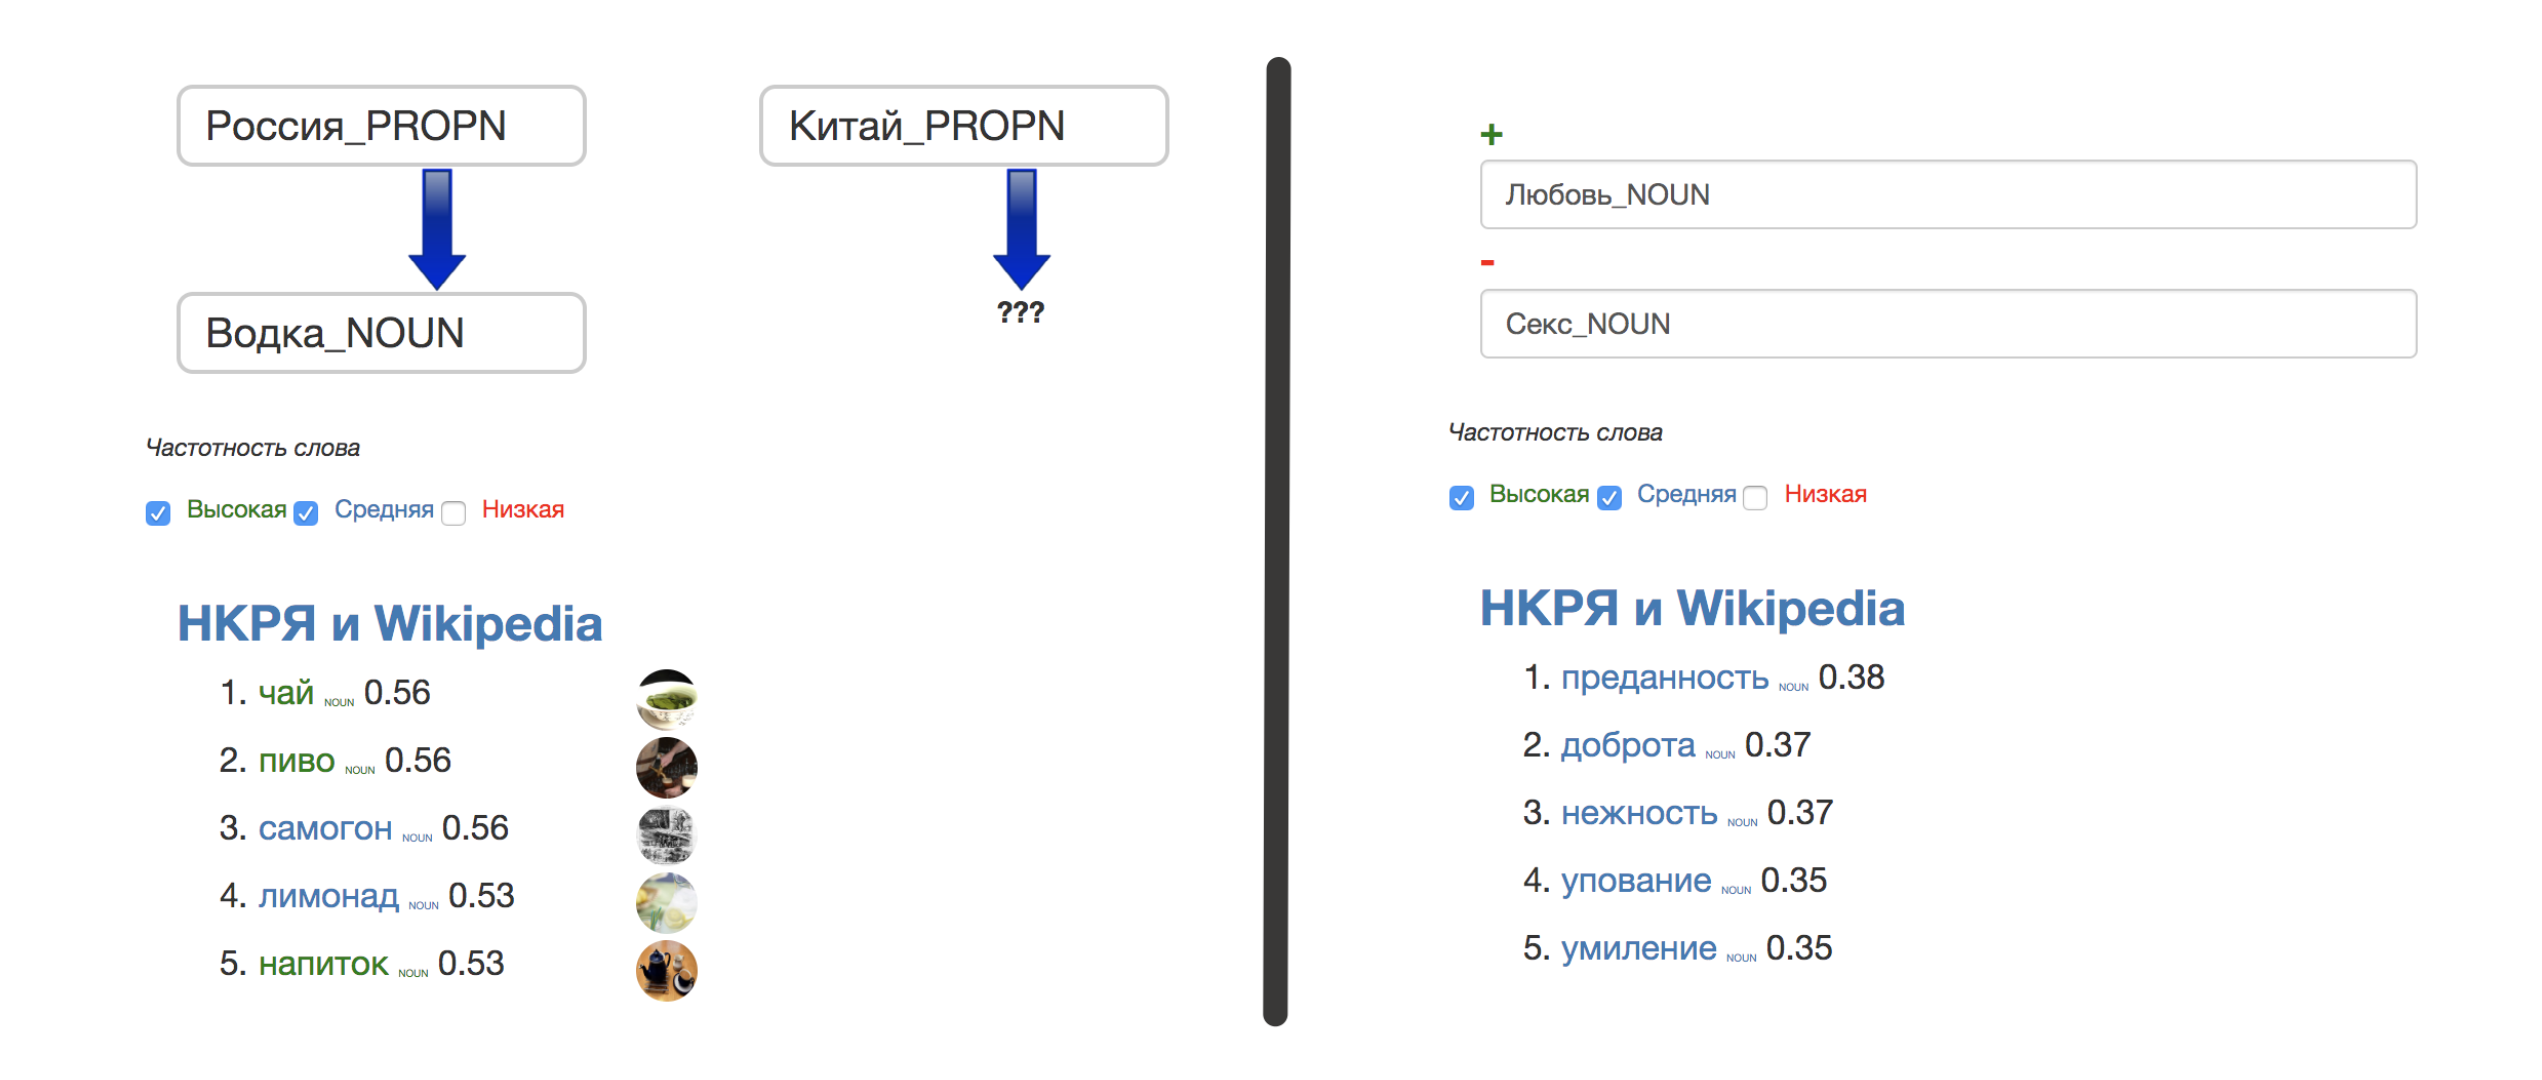
\includegraphics[width=.85\linewidth]{rusvec_calc2.png}
	\end{center}
	\vfill
	\footnotesize  {\color{blue} \url{https://rusvectores.org/ru/calculator}}
\end{frame} 


\begin{frame}{Свойства word2vec}
	Результат обучения векторных представлений сильно зависит от коллекции документов. \alert{Могут возникать неожиданные артефакты.}
	
	\begin{center}
		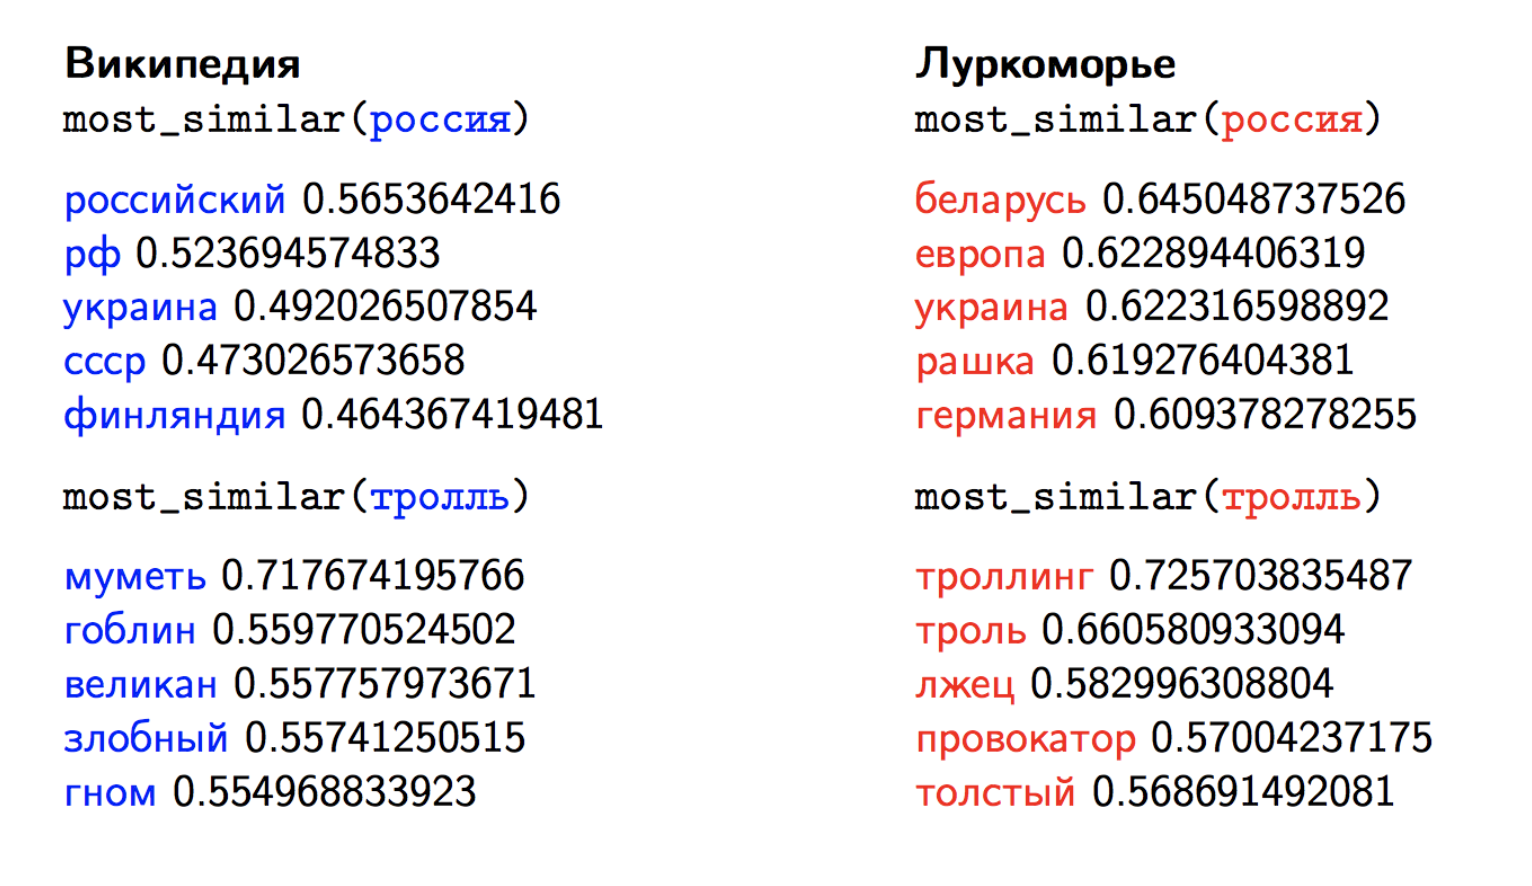
\includegraphics[width=.65\linewidth]{wikilurk.png}
	\end{center}
\end{frame} 


\begin{frame}{Word2vec всего лишь модель}
	\begin{center}
		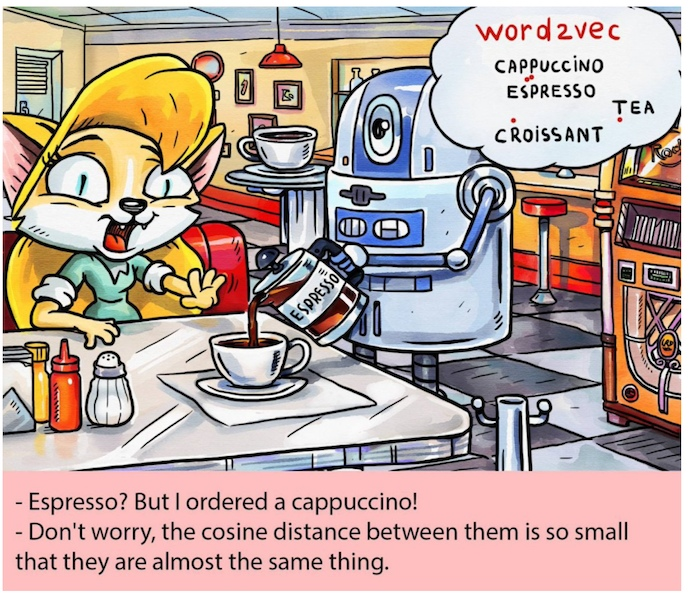
\includegraphics[width=.55\linewidth]{w2v_idiot.jpg}
	\end{center}
\end{frame} 


\begin{frame}{Как это использовать}
	\begin{wideitemize} 
		\item Можно искать похожие слова
		
		\item  Можно менять формы слов
		
		\item  Можно искать определённые отношения
		
		\item  Можно использовать как признаки для моделей
		
		\item  Обучение w2v — аналог transfer learning, но обучение идёт на фиктивную задачу, разметка, сделанная вручную, не нужна
	\end{wideitemize} 
\end{frame} 


\begin{frame}{Проблемы word2vec}
	\begin{wideitemize} 
		\item Не умеем работать с новыми словами, которых не было в нашем словаре при обучении
		
		\item  Не закладываем никакой априорной информации о разных
		формах одного слова
		
		\item  Обучаемся на контекст слова, но всё ещё действуем в парадигме мешка слов, никак не учитываем порядок слов
		
		\item Не учитываем структуру слов, не умеем обрабатывать опечатки	
	\end{wideitemize} 
\end{frame} 


\begin{frame}{Как обобщить результат до текста}
	\begin{wideitemize} 
		\item  Усреднить
		\item  Засунуть матрицу в свёрточную сетку или RNN
	    \item   doc2vec 
	\end{wideitemize} 
\end{frame} 


\begin{frame}{doc2vec (Distributed Memory)}
	\begin{center}
		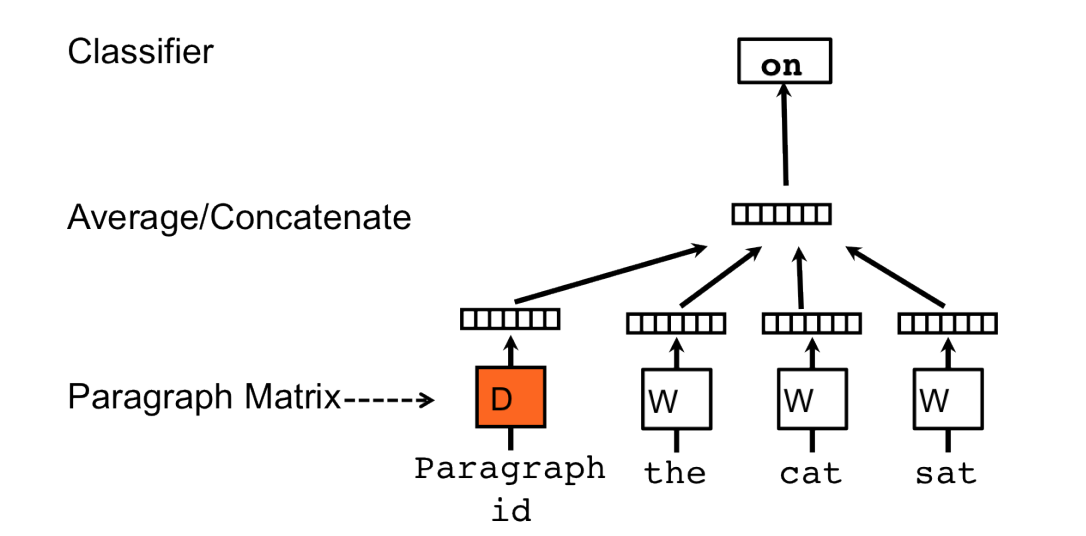
\includegraphics[width=.75\linewidth]{doc2vec1.png}
	\end{center}
	\vfill
\footnotesize  {\color{blue} \url{https://arxiv.org/abs/1405.4053}}
\end{frame} 


\begin{frame}{doc2vec (Distributed Bag Of Words)}
	\begin{center}
		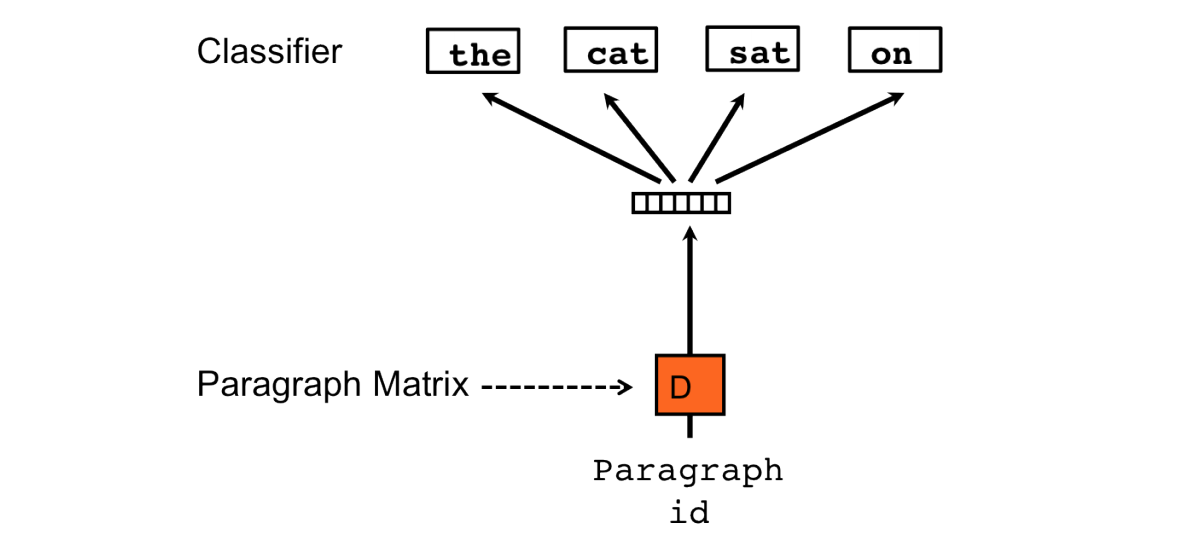
\includegraphics[width=.8\linewidth]{doc2vec2.png}
	\end{center}
	\vfill
\footnotesize  {\color{blue} \url{https://arxiv.org/abs/1405.4053}}
\end{frame} 


\begin{frame}{doc2vec}
	\begin{wideitemize} 
		\item  Инициализируем случайно дополнительный вектор для каждого параграфа или текста
		\item \alert{Distributed Memory:}  Предсказываем слово, используя вектор параграфа и контест
		\item  \alert{Distributed Bag Of Words:} предсказываем пропущенные слова по вектору документа
		\item  По-прежнему мешок слов, порядок не учитывается, новые слова и тексты не обрабатываются
	\end{wideitemize} 
	\vfill
\footnotesize  {\color{blue} \url{https://arxiv.org/abs/1405.4053}}
\end{frame} 


\begin{frame}{Fasttext} 
	\begin{wideitemize}
		\item  Усовершенствование word2vec дополнительными токенами, отвечающими за буквенные n-граммы, это решает проблему OOV (out of the vocabulary)
		\item  Например, триграмы для eating:  <ea, eat, ati, tin, ing ng>
		\item  Символы < и > это спец-символы, говорящие о том, что слово
		кончилось или началось
		\item При расчёте для слова итогового вектора будем усреднять эмбединг для слова и эмбединги для n-грамм
	\end{wideitemize}
	\vfill
	\footnotesize  {\color{blue} \url{https://arxiv.org/pdf/1607.04606v1.pdf }} \hfill \color{blue} \url{https://fasttext.cc/ } \newline 
	\color{blue} \url{https://arxiv.org/pdf/1607.01759.pdf } \hfill  \color{blue} \url{https://fasttext.cc/docs/en/crawl-vectors.html} \newline 
\end{frame}


\begin{frame}{Fasttext} 
	\begin{center}
	      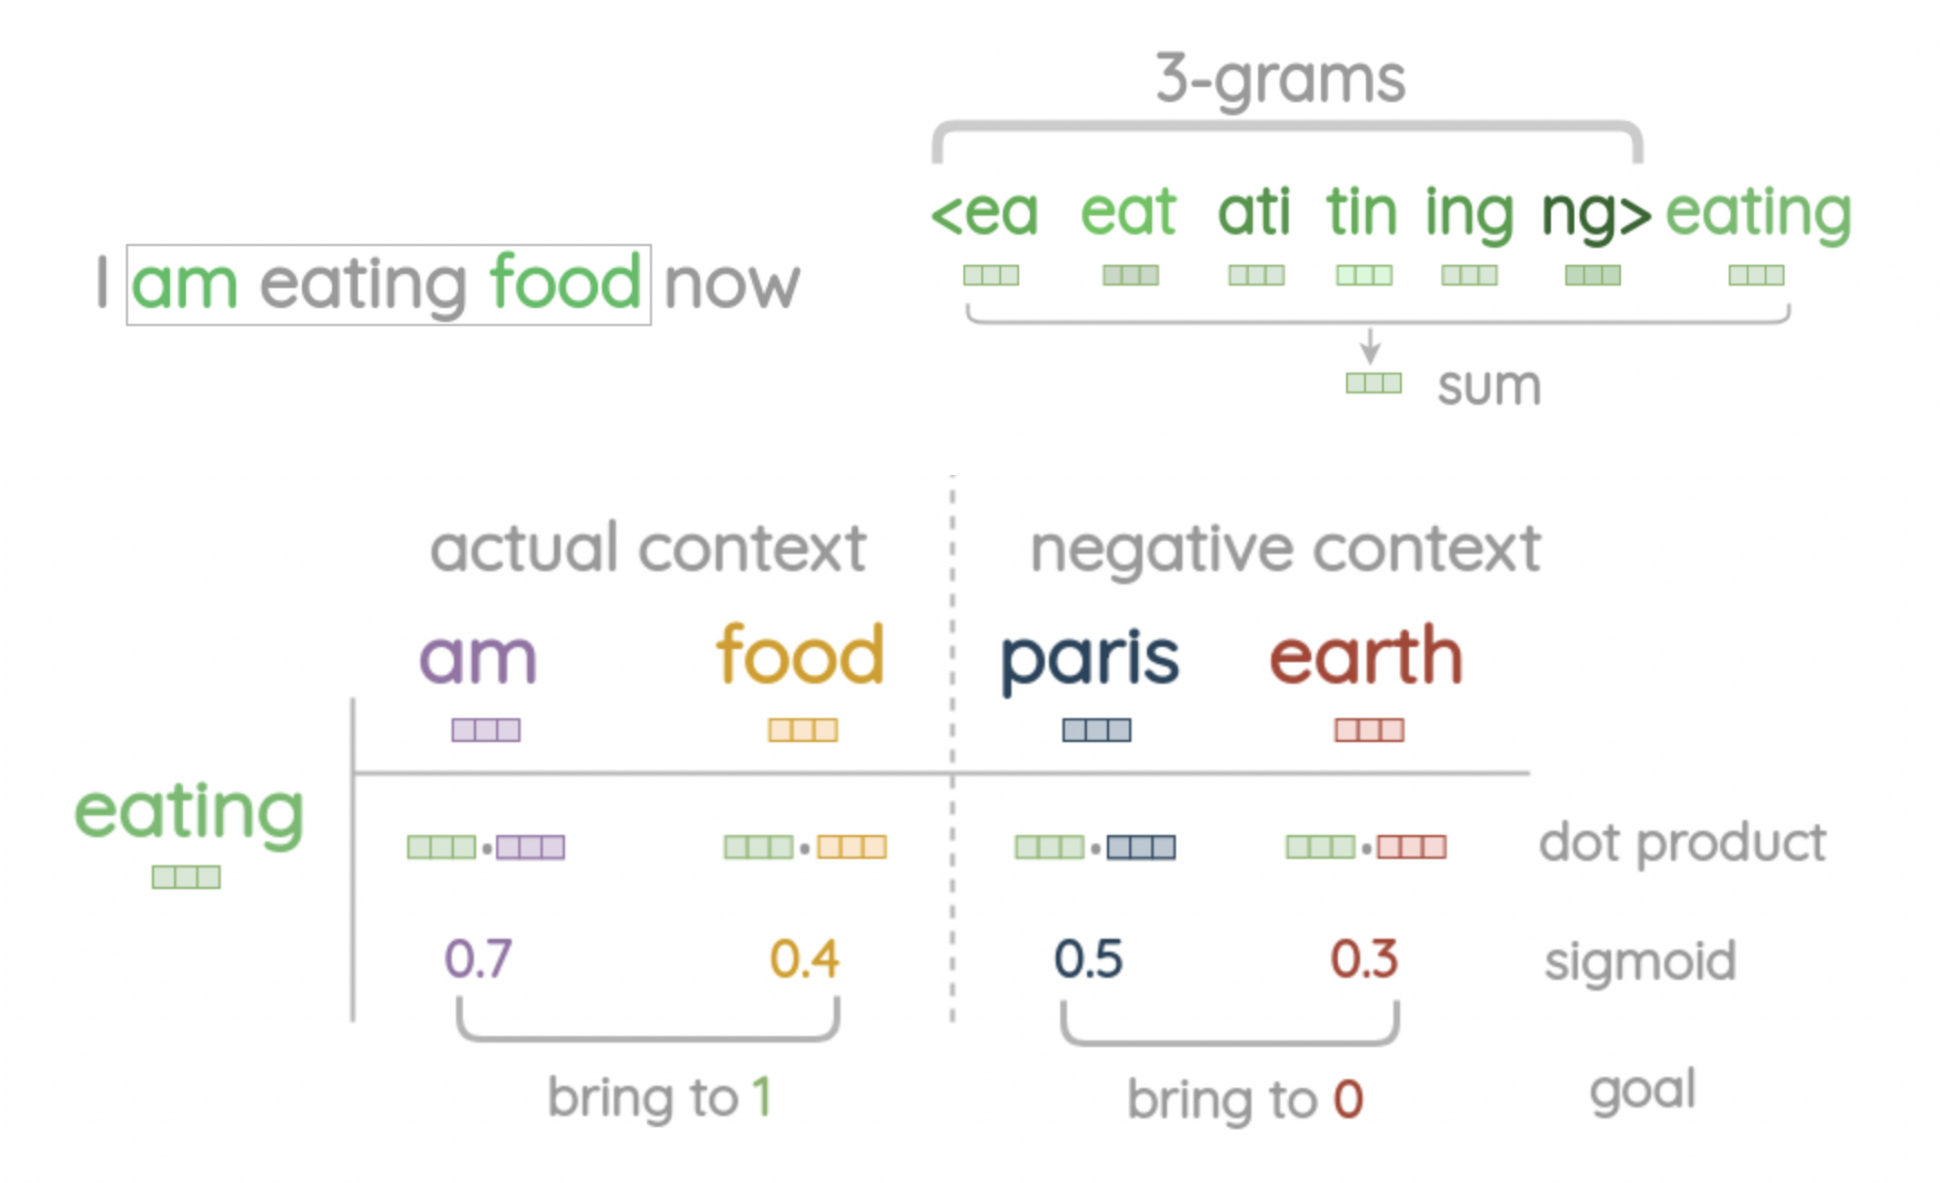
\includegraphics[width=.78\linewidth]{fasttext.png}
    \end{center}
	\vfill
\footnotesize  {\color{blue} \url{https://amitness.com/2020/06/fasttext-embeddings/}}
\end{frame}



\begin{transitionframe}
	\begin{center}
		\Huge  Что мы уже знаем про обучение представлений (картинки)
	\end{center}
\end{transitionframe}


\begin{frame}{Представления с последних слоёв}
	\begin{wideitemize}
		\item  Выходы с последних слоёв свёрточных нейросетей являются хорошими признаковыми описаниями изображений
		\item Такие векторные представления называют \alert{эмбеддингами (embeddings)}
		\item У эмбеддингов нет чёткой интерпретации, цифры в них говорят о наличии каких-то паттернов, на которые настроилась нейросетка
		\item Эмбеддинги картинок оказываются полезными во многих задачах 
	\end{wideitemize}
\end{frame}


\begin{frame}{TSNE для CIFAR-10 (предпоследний слой простой свёрточной сетки)}
		\begin{center}
				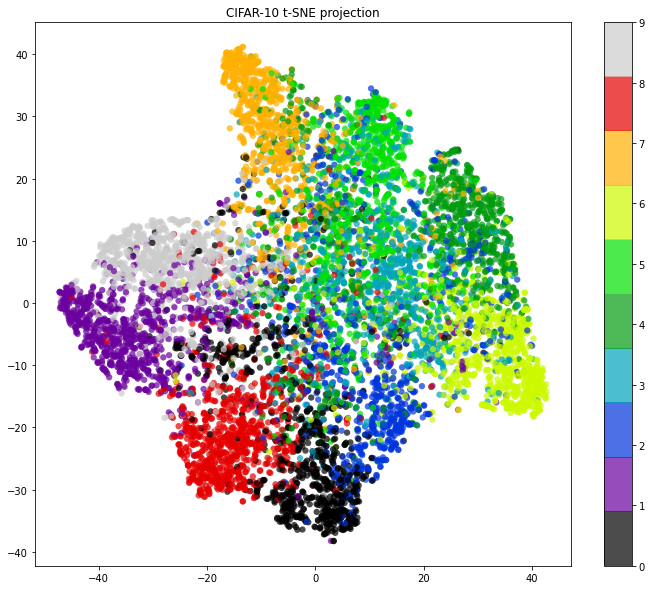
\includegraphics[width=.5\linewidth]{tsne_conv.png}
		\end{center}
\end{frame}


\begin{frame}{Представления изображений}
		\begin{center}
				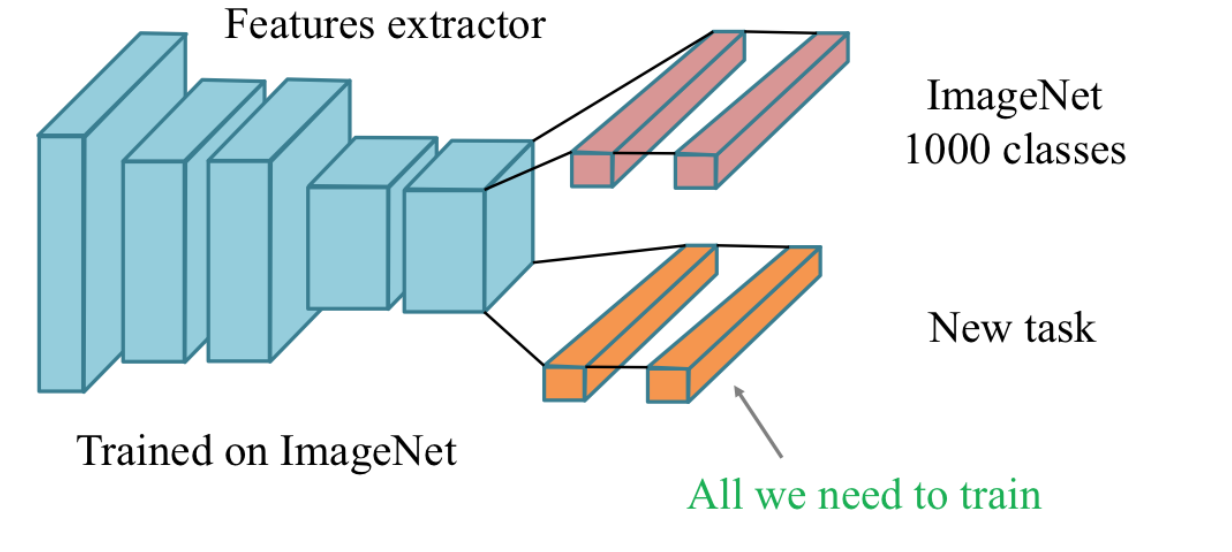
\includegraphics[width=.8\linewidth]{transfer_learning2.png}
		\end{center}
\end{frame}


\begin{frame}{Дообучение (Transfer learning)}
		\begin{wideitemize}
			\item Если данных совсем мало
			\item Берём модель из другой задачи
			\item Заменяем последний слой на слой с нужным числом выходов
			\item Обучаем только его
			\item По сути, это обучение линейной модели на эмбединге картинки
			\item Иногда приходится дообучать часть экстрактора эмбедингов
		\end{wideitemize}
\end{frame}


\begin{frame}{Представления изображений}
\begin{wideitemize}
	\item  Выход предпоследнего полносвязного слоя — хорошее
	представления картинки
	\item  Но для его обучения нужны изображения с разметкой
	\item  Может, получится строить такие представления и без разметки?	
	\item  Ведь для текстов получилось, мы собрали w2v
	\item  Нужна какая-то фейковая задача
\end{wideitemize}
\end{frame}


\begin{transitionframe}
	\begin{center}
		\Huge  Автокодировщики для картинок
	\end{center}
\end{transitionframe}


\begin{frame}{Автокодировщики}
	\begin{center}
			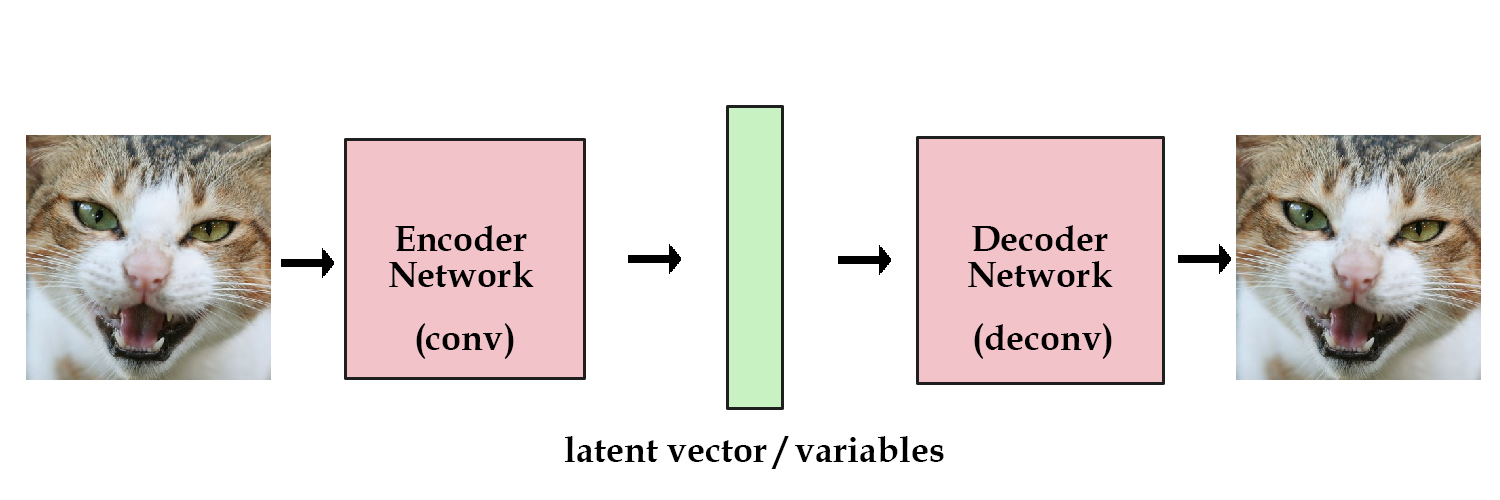
\includegraphics[width=.9\linewidth]{autoencoder.png}
		\end{center}
\end{frame}


\begin{frame}{Автокодировщики}
		\begin{center}
			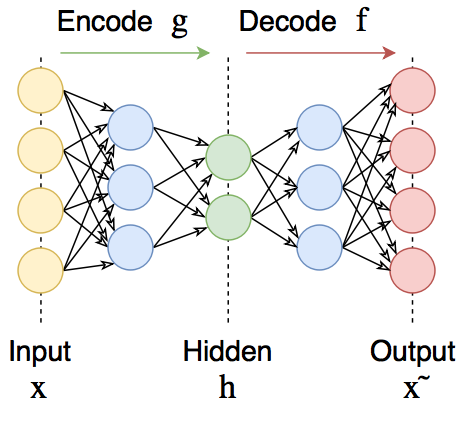
\includegraphics[width=.42\linewidth]{auto.png}
		\end{center} \pause
		\[
		\frac{1}{n} \sum_{i=1}^n L(x_i, f(g(x_i))) \to \min 
		\]
\end{frame}


\begin{frame}{Пример сжатия}
	\begin{center}
			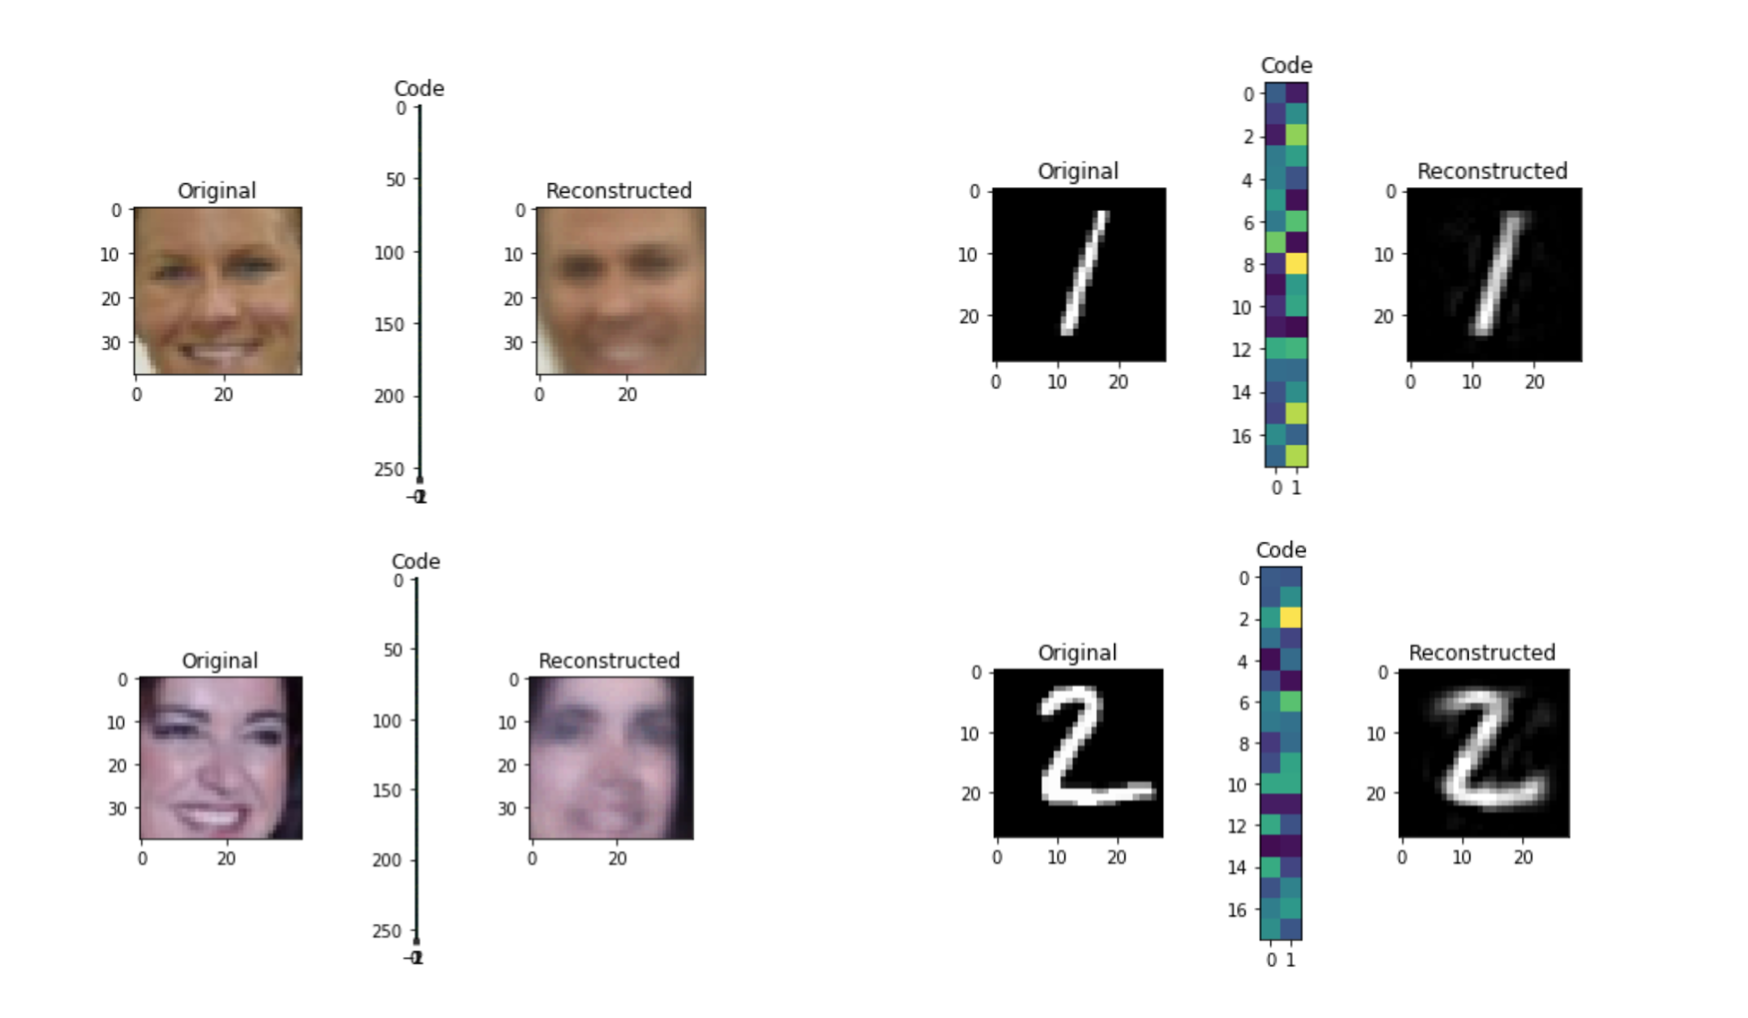
\includegraphics[width=.8\linewidth]{ato_enc.png}
		\end{center}
\end{frame}

\begin{frame}{Зачем это всё?}
\begin{wideitemize}
	\item  Сжатие данных (нелинейных аналог PCA)
	\item  Очистка картинки от шума
	\item  Поиск похожих изображений
	\item  Трансформация изображений
	\item  Генерация изображений
\end{wideitemize}
\end{frame}


\begin{frame}{Автокодировщики}
\begin{wideitemize}
	\item  Понижают размерность, исходная картинка восстанавливается с потерями
	\item  Основная ценность — эмбединг из булочного горлышка, хочется чтобы он получился максимально качественным
	\item  Наша архитектура сильно переобучается под выборку, для новых лиц работает хуже
	\item  Нужна регуляризация, которая позволит извлекать смысл, а не восстанавливать пиксели в точности (фон тоже запоминается)
\end{wideitemize}
\end{frame}


\begin{frame}{Что находит нейросеть... опять ...}
	\begin{center}
			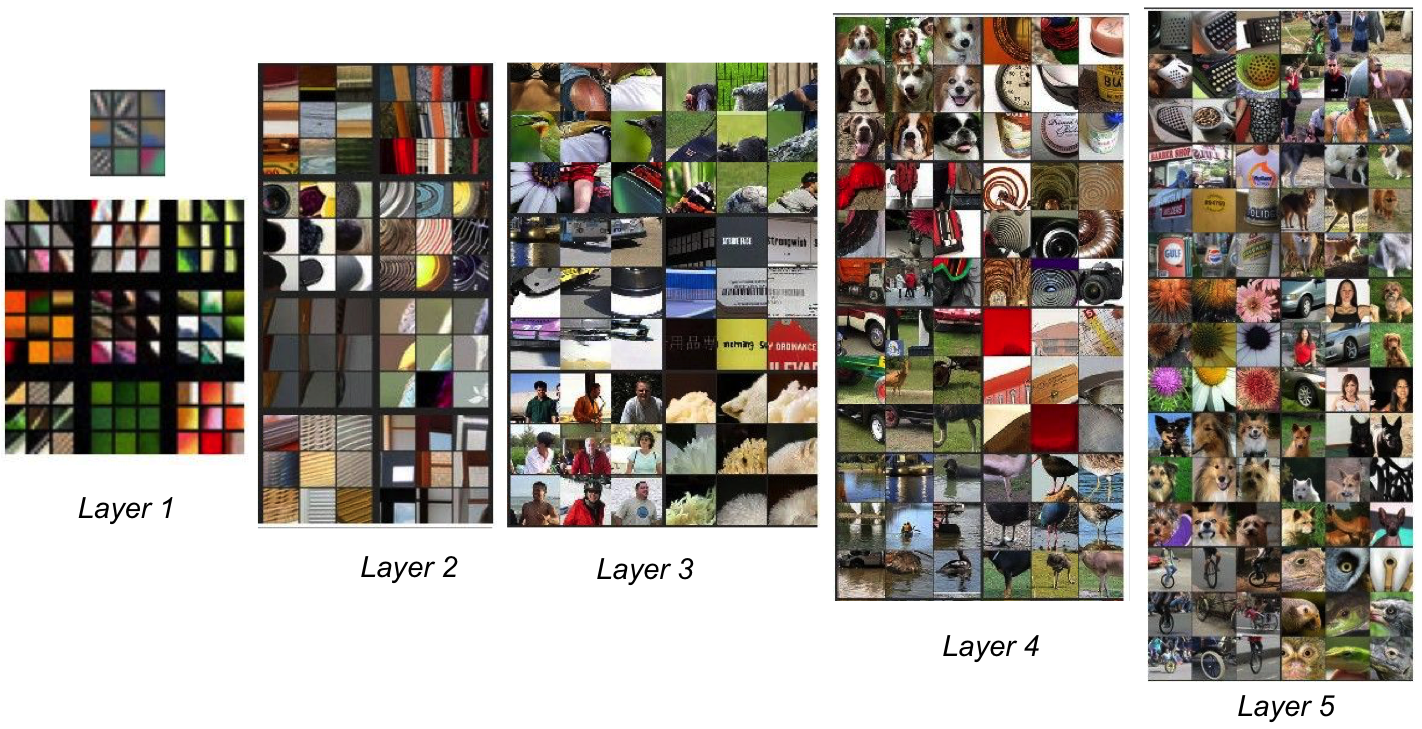
\includegraphics[width=.85\linewidth]{cnn_vis.png}
		\end{center}
\end{frame}


\begin{frame}{Perceptual loss}
	\begin{center}
			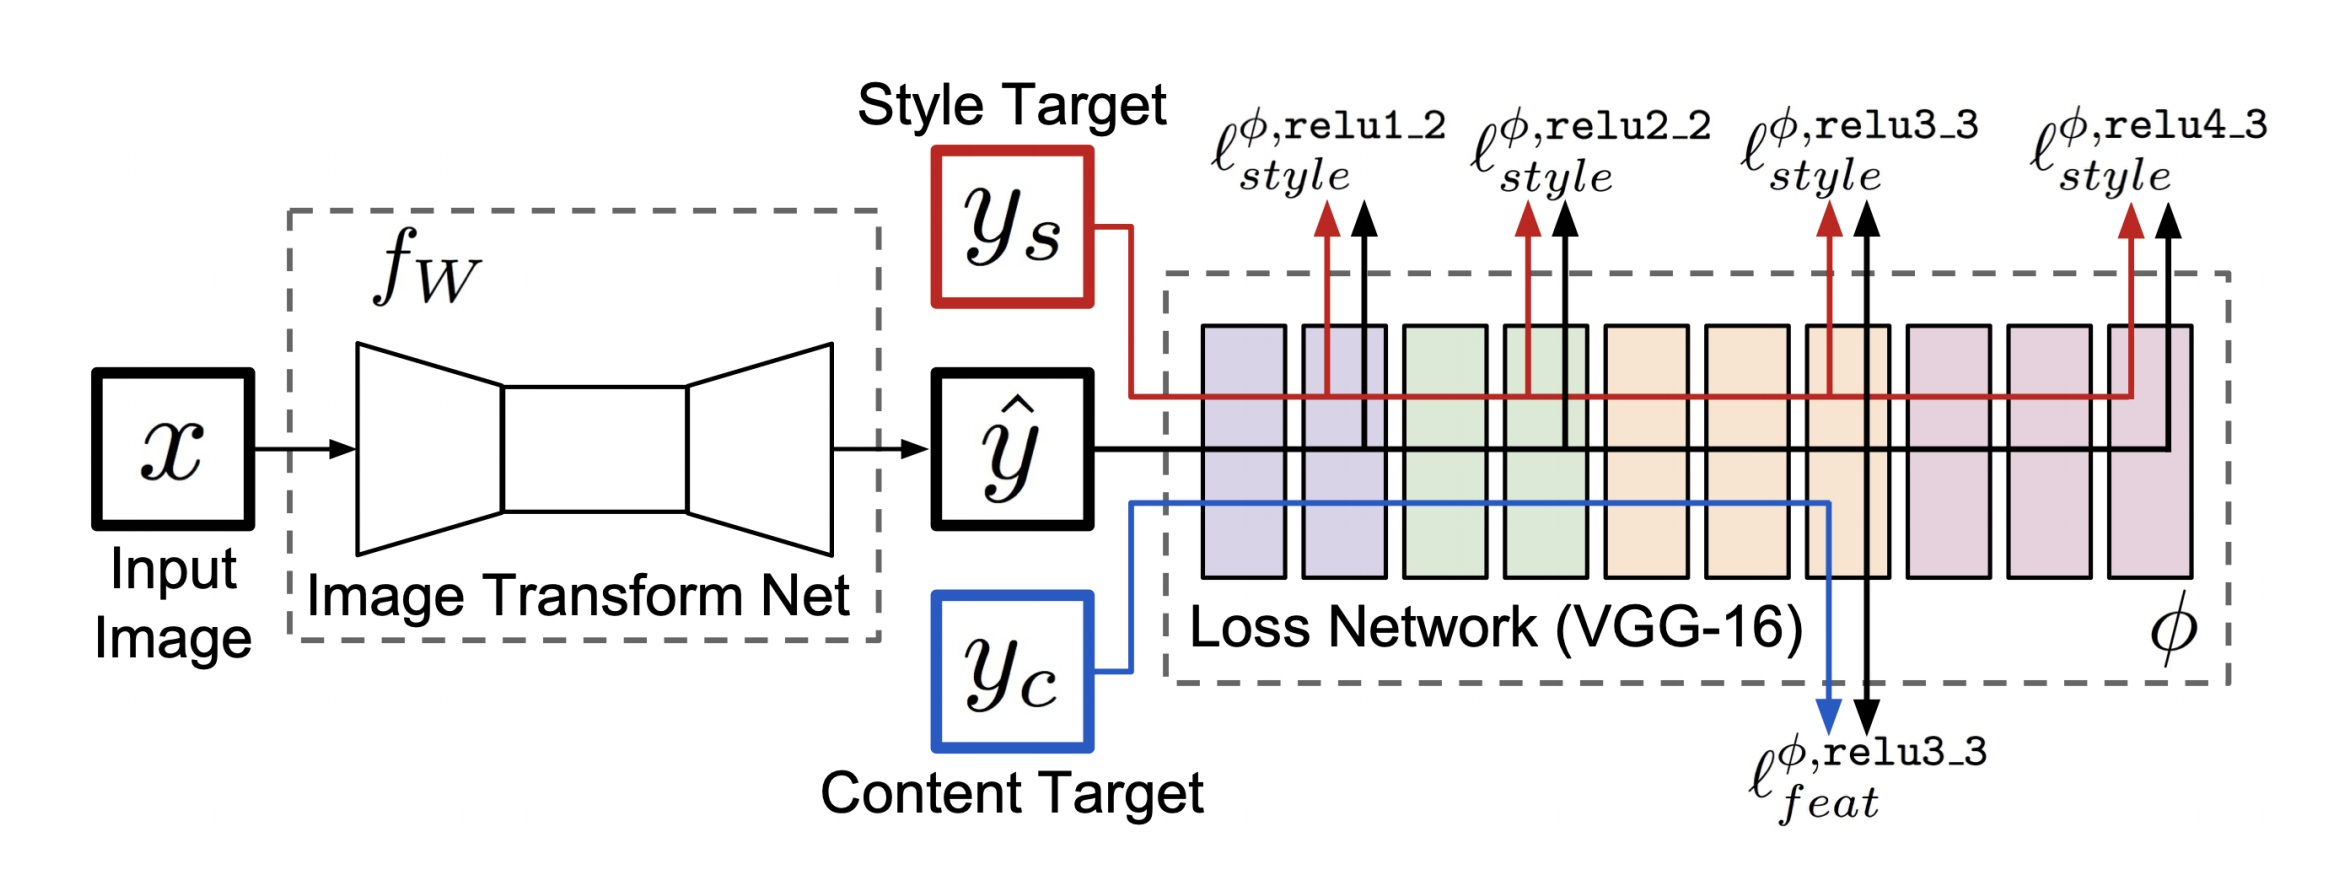
\includegraphics[width=.8\linewidth]{perceptual_loss.png}
		\end{center}
	\vfill
	\footnotesize
	{\color{blue} \url{https://arxiv.org/pdf/1603.08155.pdf}} 
\end{frame}


\begin{frame}{Perceptual loss}
\begin{wideitemize}
	\item  Чем глубже слой, тем осмысленнее образы
	\item  Ранние слои во многом определяют стиль картинки
	\item  Можно измерять расстояния между выходами свёрточных слоёв картинок
	\item  Это поможет сохранить смысл и сделать эмбединг более осмысленным
\end{wideitemize}
	\vfill
\footnotesize
{\color{blue} \url{https://arxiv.org/pdf/1603.08155.pdf}} 
\end{frame}


\begin{frame}{Denoising autoencoder}
\begin{center}
	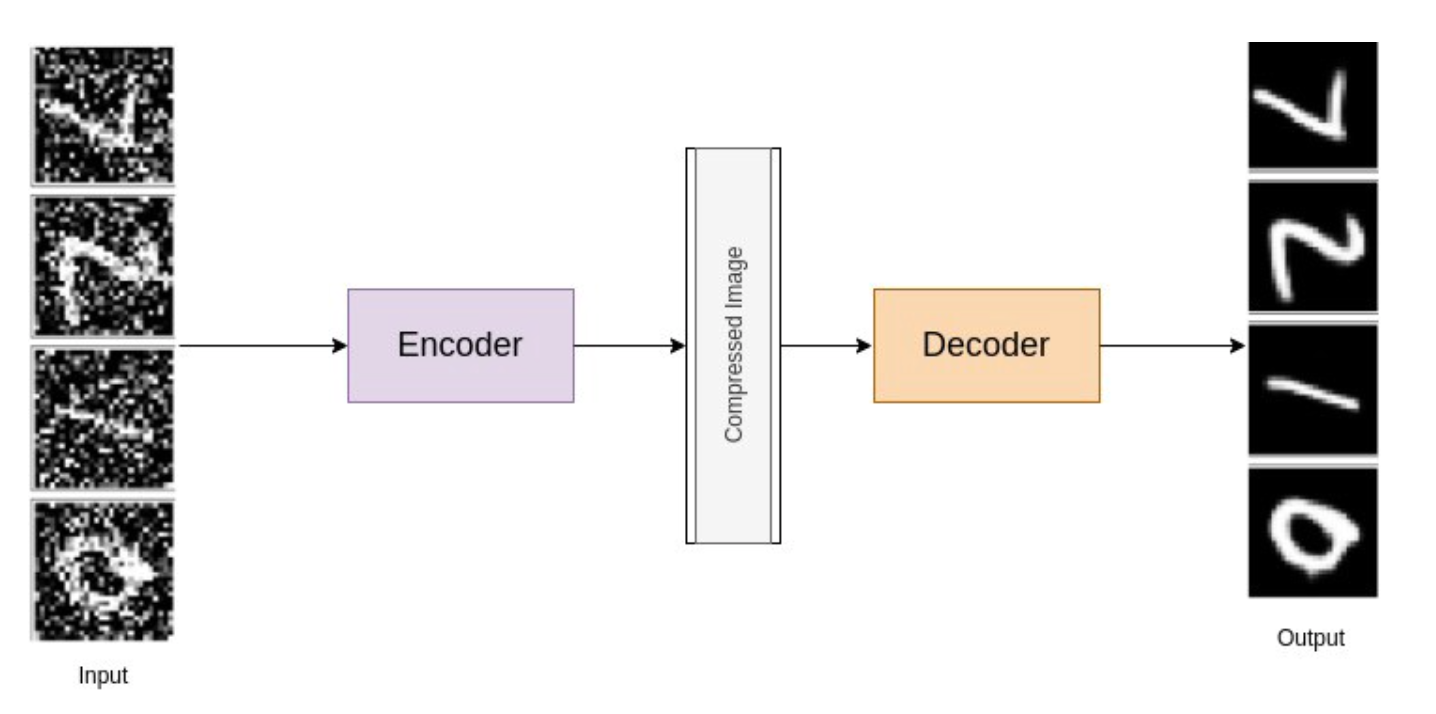
\includegraphics[width=.8\linewidth]{denoise.png}
\end{center}
\vfill
\footnotesize
{\color{blue} \url{https://medium.com/@garimanishad/reconstruct-corrupted-data-using-denoising-autoencoder-python-code-aeaff4b0958e} \newline \url{https://www.cs.toronto.edu/~larocheh/publications/icml-2008-denoising-autoencoders.pdf} } 
\end{frame}


\begin{frame}{Morphing faces}
\begin{center}
	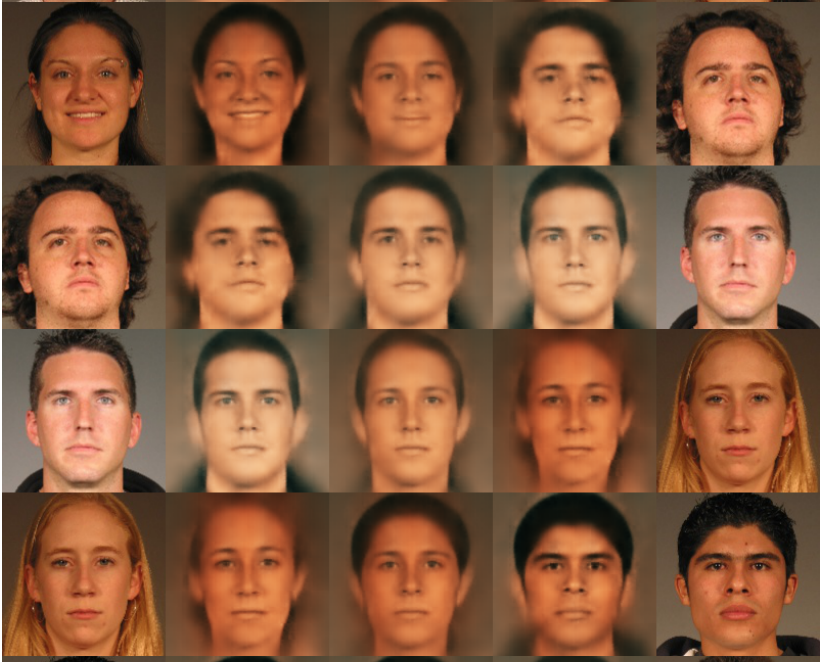
\includegraphics[width=.5\linewidth]{morth.png}
\end{center}
\vfill
\footnotesize
{\color{blue} \url{http://essay.utwente.nl/81372/1/Heuver_MA_EEMCS.pdf}  } 
\end{frame}


\begin{frame}{Morphing faces}
\begin{center}
	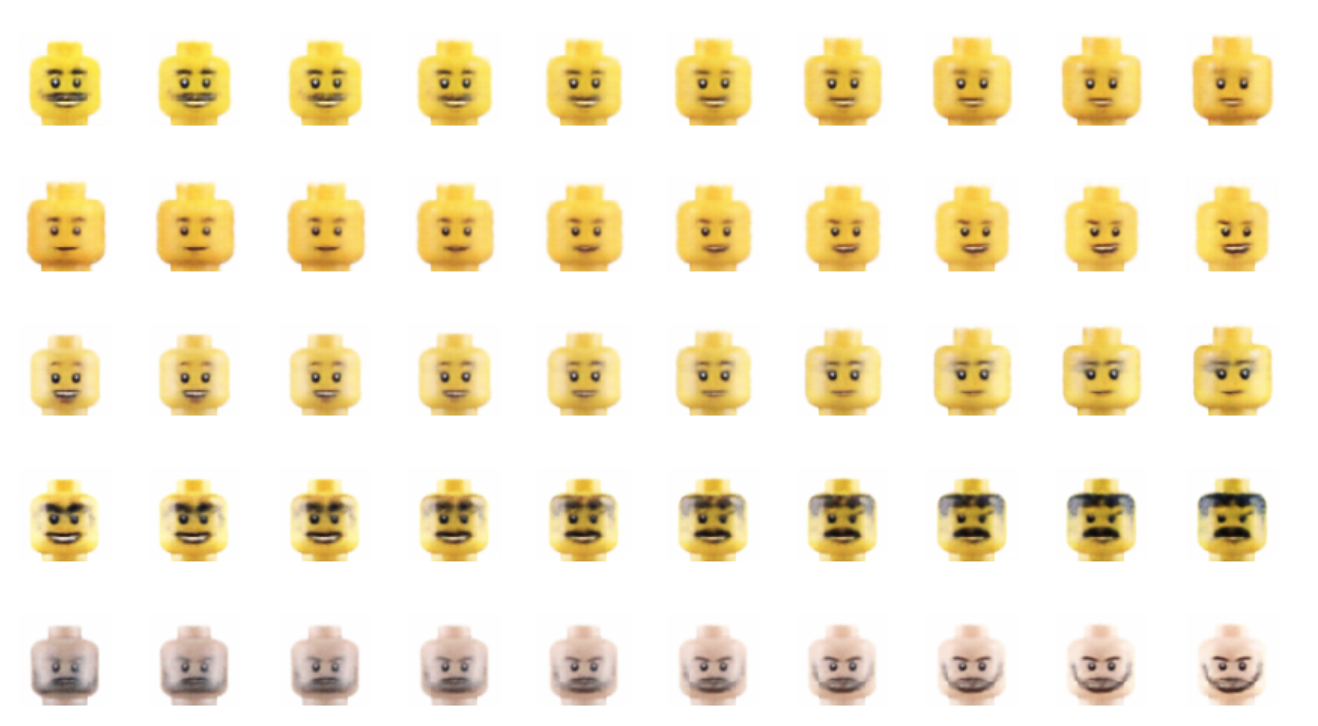
\includegraphics[width=.85\linewidth]{lego.png}
\end{center}
\vfill
\footnotesize
{\color{blue} \url{https://www.echevarria.io/blog/lego-face-vae/index.html}  } 
\end{frame}


\begin{frame}{Саморегуляция выборки}
\begin{center}
	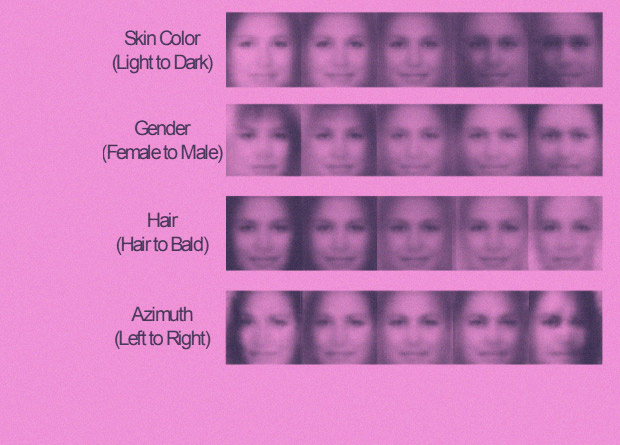
\includegraphics[width=.6\linewidth]{avtoreg.png}
\end{center}
\vfill
\footnotesize
{\color{blue} \url{https://nplus1.ru/news/2019/01/28/debiasing-faces}  } 
\end{frame}


\begin{frame}{Поиск фрода}
\begin{center}
	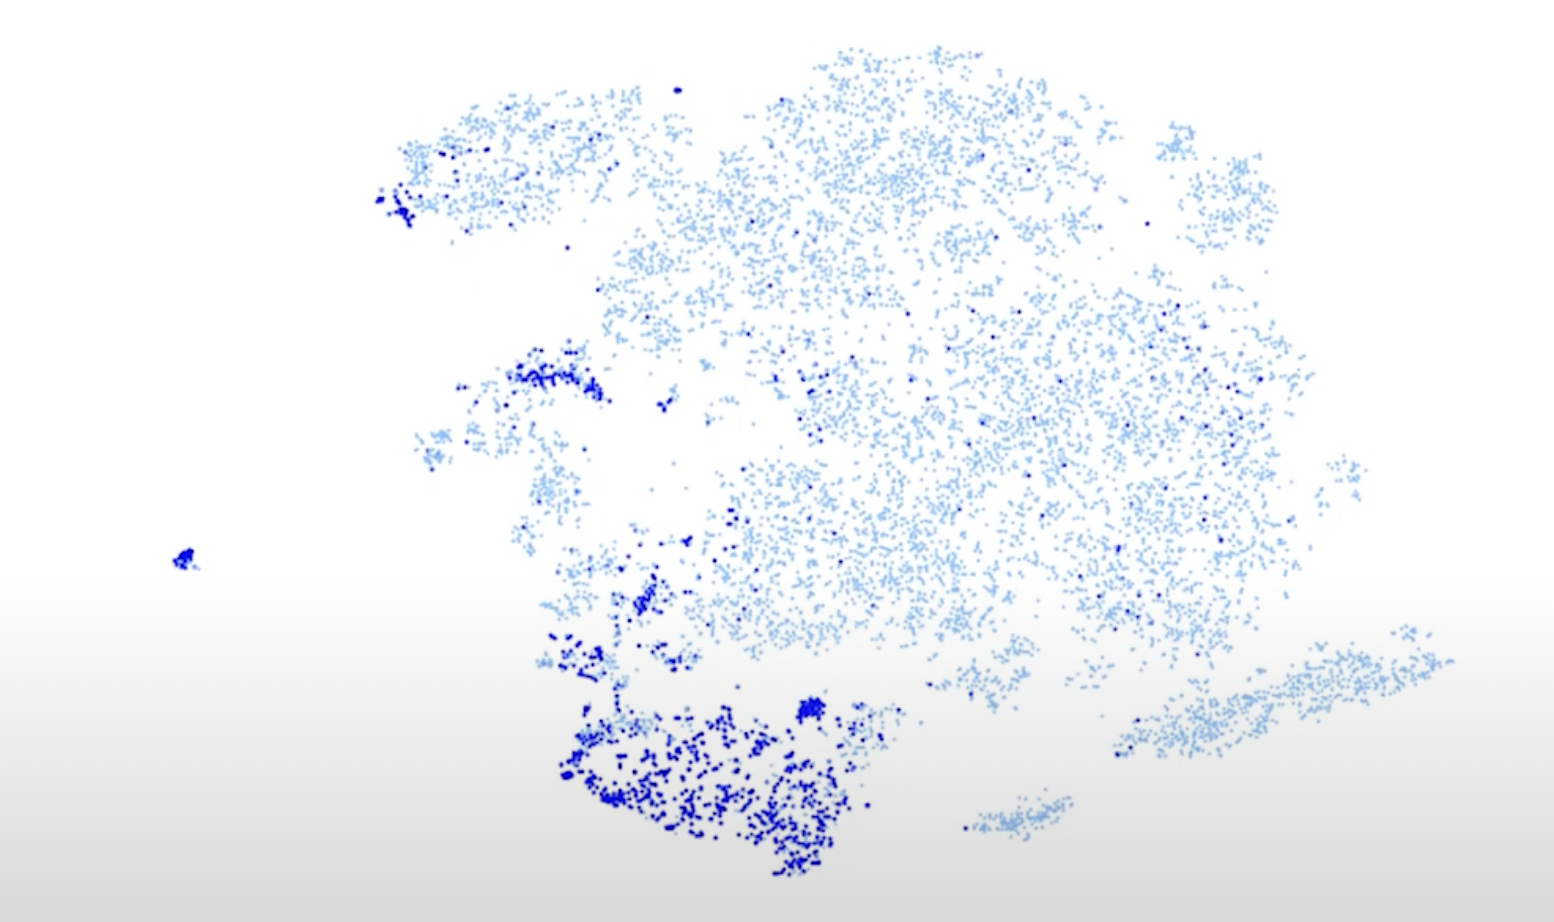
\includegraphics[width=.7\linewidth]{yandex_tsne.png}
\end{center}
\vfill
\footnotesize
Автокодировщики в антифроде Яндекса: {\color{blue} \url{https://www.youtube.com/watch?v=aBckDgtG0Zs}  } 
\end{frame}



\begin{transitionframe}
	\begin{center}
		\Huge  Обучение представлений для графов
	\end{center}
\end{transitionframe}


\begin{frame}{Задачи на графах}
	\begin{wideitemize}
		\item  \alert{Node-focused tasks:}  изучаем структурные свойства вершина графа относительно других вершин 
		
		\item классификация вершин (поиск хабов в транспортных сетях), предсказание связей (предсказания взаимодействия между белками), рекомендация вершин (поиск возможных друзей в социальных сетях)
		
		\item  \alert{Graph-focused tasks:}  изучаем граф целиком или подграф
		
		\item  классификация графов (предсказание токсичности молекулы), генерация графов (генерация молекул белков с желаемыми свойствами)
		
	\end{wideitemize}
	\vfill
	\footnotesize
	{\color{blue} \url{https://github.com/esokolov/ml-course-hse/blob/master/2021-spring/seminars/sem17-graph.pdf}  } 
\end{frame}


\begin{frame}{Представления для вершин}
	\begin{wideitemize}
		\item  Обучаем векторное представление вершин графа, хотим чтобы вектор включал в себя информацию о структурной роли вершина графа
		
		\item  Граф:  $\mathcal{G} = (\mathcal{V}, \mathcal{E})$ 

		\item  Множество вершин:  $\mathcal{V} = \{v_i\}_{i=1}^{|\mathcal{V}|}$ 
		
		\item  Ребра с неотрицательными весами: $\mathcal{E}: \mathcal{V}\times\mathcal{V}\to\mathbb{R}_{\ge 0}$
		
		\item  Функция похожести между вершинами:  $s_{\mathcal{G}}: \mathcal{V}\times\mathcal{V}\to\mathbb{R}$

	\end{wideitemize}
\end{frame}


\begin{frame}{Примеры функции похожести между вершинами}
	\begin{wideitemize}
		\item   Если вершины соединены ребром $s_{\mathcal{G}}(v_i, v_j)=1$ и $s_{\mathcal{G}}(v_i, v_j)=0$ иначе
	
		\item   Формула, зависящая от растояния между вершинами
		
		$$
		s_{\mathcal{G}}(v_i, v_j) = \exp\left(-\frac{d_{\mathcal{G}}(v_i, v_j)}{\tau}\right),
		$$
		
		где $d_{\mathcal{G}}(v_i, v_j)$ — расстояние между вершинами $v_i$ и $v_j$, а $\tau$ — гиперпараметр. 
		
		\item  Оценить вероятность перехода из одной вершины в другую случайным блужданием по графу
				
	\end{wideitemize}
\end{frame}


\begin{frame}{Энкодер и декодер для графов}
	\begin{wideitemize}
		\item  Энкодер преобразует данные в вектор размерности $d$:
		
		\[ \ENC: \mathcal{V} \to \mathbb{R}^d, \ENC(v_i)=z_i \]
		
		\item  Декодер принимает два векторных представления и пытается приблизить функцию похожести сответствующих вершин:
		
		\[ \DEC: \mathbb{R}^d \times \mathbb{R}^d \to \mathbb{R}, \DEC(z_i, z_j)\approx s_{\mathcal{G}}(v_i, v_j) \]
		
		\item Для обучения берём удобную функцию потерь и минимизируем по параметрам декодера и энкодера: 
		
		\[  \sum_{v_i, v_j \in \mathcal{V}} \mathcal{L} \bigg(\DEC\Big(\ENC(v_i), \ENC(v_j)\Big), s_{\mathcal{G}}(v_i, v_j)\bigg) \to \min_{\ENC, \DEC} \]
	\end{wideitemize}
\end{frame}


\begin{frame}{Пример:}
	\begin{wideitemize}
			\item В качестве энкодера в простейшем случае можем взять матрицу  $|\mathcal{V}| \times d$
			
			\item В роли декодера можно использовать обычное скалярное произведение  $\DEC(z_i, z_j) = z_i^T z_j$
	\end{wideitemize}
\end{frame}


\begin{frame}{node2vec}
	\begin{wideitemize}
		\item  В качестве функции похожести используем вероятность случайного блуждания  попсть из вершины $v_i$ в вершину $v_j$ ,   $p(v_j|v_i)$
		
		\item Будем обучать вектора так, чтобы 
		
		\[ p(v_j|v_i) \approx \frac{e^{z_j^T z_i}}{\sum_k e^{z_k^T z_i}} = \DEC(z_i, z_j) \]
		
		\item Энкодер тут матрица, а декодер Softmax от скалярных произведений  \pause 
		
		\item  Для оценки вероятностей будем запускать по графу случайные блуждания из разных вершин какой-то длины  \pause 
		
		\item  \alert{Узнали word2vec ???}  Фактически это skip-gram word2vec, где словами являются вершины графа, а предложениями случайные пути в графе
	\end{wideitemize}
\end{frame}


\begin{frame}{node2vec}

	\begin{center}
		\begin{tikzpicture}[scale=0.7,
			roundnode/.style={circle, draw=black, thick, minimum size=10mm}
			]
			
			\node[roundnode, fill=orange] at (-2, 4) (3) {$v_3$};
			\node[roundnode, fill=orange] at (0.5, 3.5) (4) {$v_4$};
			\node[roundnode, fill=orange] at (-2.5, 0.5) (1) {$v_1$};
			\node[roundnode] at (-1.5, 2) (2) {$v_2$};
			\node[roundnode, fill=orange] at (0, 0) (5) {$v_5$};
			\node[roundnode, fill=orange] at (2, 2) (6) {$v_6$};
			\node[roundnode, fill=orange] at (3.5, 0.5) (8) {$v_8$};
			\node[roundnode, fill=orange] at (5, 2.5) (9) {$v_9$};
			\node[roundnode] at (6, 0) (10) {$v_{10}$};
			\node[roundnode, fill=orange] at (3, 4) (7) {$v_7$};
			\node[roundnode] at (7, 3.5) (11) {$v_{11}$};
			
			\draw[->, thick] (1.east) -- (5.west);
			\draw[->, thick] (5.north east) -- (6.south west);
			\draw[->, thick] (6.north) -- (7.south west);
			\draw[->, thick] (7.south east) -- (9.north west);
			\draw[->, thick] (9.south west) -- (8.north east);
			\draw[->, thick] (8.north west) -- (6.south east);
			\draw[->, thick] (6.north west) -- (4.south east);
			\draw[->, thick] (4.west) -- (3.east);
			
			\draw[-, dashed, thick] (1.north) -- (2.south west);
			\draw[-, dashed, thick] (2.north west) -- (3.south);
			\draw[-, dashed, thick] (2.north east) -- (4.south west);
			\draw[-, dashed, thick] (2.south east) -- (5.north west);
			\draw[-, dashed, thick] (4.south) -- (5.north);
			\draw[-, dashed, thick] (4.east) -- (7.west);
			\draw[-, dashed, thick] (5.east) -- (8.west);
			\draw[-, dashed, thick] (6.east) -- (9.west);
			\draw[-, dashed, thick] (7.east) -- (11.north west);
			\draw[-, dashed, thick] (8.east) -- (10.west);
			\draw[-, dashed, thick] (9.north east) -- (11.west);
			\draw[-, dashed, thick] (9.south east) -- (10.north);
			\draw[-, dashed, thick] (10.north east) -- (11.south);
		\end{tikzpicture}
	\end{center}

\only<1>{
\begin{itemize}
	\item  Случайный путь: $ S=[v_1, v_5, v_6, v_7, v_9, v_8, v_6, v_4, v_3] $
	\item  Пусть размер контекста равен $2$
	\item  Для $v_1$ получаем $[\underline{v_1}, v_5, v_6]$
	\item  Для первого вхождения $v_6$ получим $[v_1, v_5, \underline{v_6}, v_7, v_9]$
\end{itemize}}

\only<2>{
	\begin{itemize}
		\item  Для каждого окна выписываем пары (центр окна, другое упоминание вершины в окне)
		\item  Для  $[v_1, v_5, \underline{v_6}, v_7, v_9]$ получаем  пары $(v_6, v_1)$, $(v_6, v_5)$, $(v_6, v_7)$, $(v_6, v_9)$. 
\end{itemize}}


\only<3>{
	\begin{itemize}
		\item Минимизируем функционал:
		$$
		\mathcal{L} = \sum_{(v_i, v_j)} -\log \big(\DEC(z_i, z_j)\big) = \sum_{(v_i, v_j)} \Big(-z_j^T z_i + \log \sum_k e^{z_k^T z_i} \Big) \to \min_{z}
		$$
		\item Вместо софтмакса обычно делают негативное сэмплирование 
	\end{itemize}}
\end{frame}



\begin{frame}{node2vec}
	\begin{wideitemize}
		\item  Итоговые векторы будут содержать информацию о близости вершин с точки зрения случайного блуждания, его можно параметризовать
	\end{wideitemize}

	\begin{center}
		\begin{tikzpicture}[
			roundnode/.style={circle, draw=black, thick, minimum size=10mm},
			emptynode/.style={circle, draw=white}
			]
			
			\node[roundnode, fill=orange] at (0, 0) (1) {$v_1$};
			\node[roundnode, fill=green] at (2, 2) (2) {$v_2$};
			\node[roundnode, fill=yellow] at (-0.5, 3.5) (3) {$v_3$};
			\node[roundnode, fill=cyan] at (3.5, 4) (4) {$v_4$};
			\node[roundnode, fill=cyan] at (4.5, 0.5) (5) {$v_5$};
			
			\node[emptynode] at (-1.2, 0) (1a) {};
			\node[emptynode] at (-0.9, -0.9) (1b) {};
			\node[emptynode] at (-1.5, 4.2) (3a) {};
			\node[emptynode] at (-0.5, 4.7) (3b) {};
			\node[emptynode] at (3.5, 5.2) (4a) {};
			\node[emptynode] at (4.5, 4.7) (4b) {};
			\node[emptynode] at (5.7, 0.5) (5a) {};
			\node[emptynode] at (5.4, -0.3) (5b) {};
			
			\draw[->, thick] (1.north east) -- (2.south west);
			\draw[-, dashed, thick] (1.north) -- (3.south);
			\draw[-, dashed, thick] (2.north west) -- (3.south east);
			\draw[-, dashed, thick] (2.north east) -- (4.south west);
			\draw[-, dashed, thick] (2.south east) -- (5.north west);
			
			\draw[-, dashed, thick] (1.west) -- (1a.east);
			\draw[-, dashed, thick] (1.south west) -- (1b.north east);
			\draw[-, dashed, thick] (3.north west) -- (3a.east);
			\draw[-, dashed, thick] (3.north) -- (3b.south);
			\draw[-, dashed, thick] (4.north) -- (4a.south);
			\draw[-, dashed, thick] (4.north east) -- (4b.west);
			\draw[-, dashed, thick] (5.east) -- (5a.west);
			\draw[-, dashed, thick] (5.south east) -- (5b.north west);
			
			\node[below] at (1.45, 0.9) {$\alpha = 1/p$};
			\node[below] at (3.9, 1.8) {$\alpha = 1/q$};
			\node[below] at (3.5, 3.2) {$\alpha = 1/q$};
			\node[below] at (1, 3.4) {$\alpha = 1$};
			
		\end{tikzpicture}
	\end{center}
\end{frame}


\begin{frame}{node2vec}
	Допустим, на очередном шаге блуждания мы попали из вершины $v_1$ в вершину $v_2$. Чтобы определить вероятности перехода в соседние вершины, зададим веса ребрам $\alpha$:

	\begin{wideitemize}
		\item  Для ребра, ведущего обратно, положим $\alpha = 1/p$.
		
		\item  Для общих соседей предыдущей и текущей вершины положим $\alpha=1$.
		
		\item Для всех остальных вершин положим $\alpha = 1/q$.
		
		\item  \alert{Что контролирует $p$?}   \alert{Что контролирует $q$?} 
 	\end{wideitemize}
\end{frame}


\begin{frame}{Особенности node2vec}
	\begin{wideitemize}
		\item  Непонятно что делать с новыми вершинами, появляющимися в графе
		\item  Никак не учитываем мета-ифнормацию о вершинах
		\item  Для вершин нет общих параметров, можем переобучится
	\end{wideitemize}
\end{frame}



\begin{frame}{Neighborhood autoencoder}
	\begin{wideitemize}
		\item  Поставим в соотвествие каждой вершине вектор из её похожестей на остальные  (вектор будет очень длинный)
		\[ v_i \mapsto s_i, s_{ij} = s_{\mathcal{G}}(v_i, v_j) \]
		
		\item  Сжимаем с помощью автокодировщика
		
		\[z_i = \ENC(s_i), \DEC(z_i) \approx s_i\] 
		
		
		\item Обучать можно, например, с помощью MSE: 
		
		\[ \sum_{i} \Big\|\DEC\big(\ENC(s_i)\big) - s_i\Big\|^2 \to \min_{\ENC, \DEC} \]
	\end{wideitemize}
\end{frame}


\begin{frame}{Особенности Neighborhood autoencoder}	
	\begin{wideitemize}
		\item  Параметры модели будут общими для всех вершин
		\item  Всё ещё не умеем генерировать эмбеддинги для новых вершин
		\item  Всё ещё не используем метаданные
	\end{wideitemize}
\end{frame}


\begin{frame}{Neighborhood aggregation}
	\begin{wideitemize}
		\item  Для каждой вершины будем агрегировать признаки её соседей, в том числе метаданные ( можно их усреднять )
		\item  Соединяем вектор агрегированных признаков с признаками исходной вершины 
		\item  Обучаем на них автокодировщик
	\end{wideitemize}
\end{frame}


\begin{frame}{Представления для графов}
	\begin{wideitemize}
		\item  Усреднить эмбеддинги вершин: 
		
		$$
		z_{\mathcal{G}} = \frac{1}{|\mathcal{V}|} \sum_{v \in \mathcal{V}} z_v
		$$
		
		\item  Обрабатывать последовательность из эмбеддингов вершин рекуррентными нейросетями 
		
		\item  Изучить более продвинутые методы :) 
	\end{wideitemize}
\end{frame}


\begin{transitionframe}
	\begin{center}
			\Huge  ELMO 
	\end{center}
\end{transitionframe}


\begin{frame}{Embeddings from Language Models (ELMo)} 
	 \begin{wideitemize}
			\item  Усложним наши модели для текстов: начнём учитывать порядок слов
			\item  Для этого соберём рекуррентный автокодировщик
	\end{wideitemize}
\end{frame}


\begin{frame}{ Embeddings from Language Models (ELMo)}
	\begin{center}
			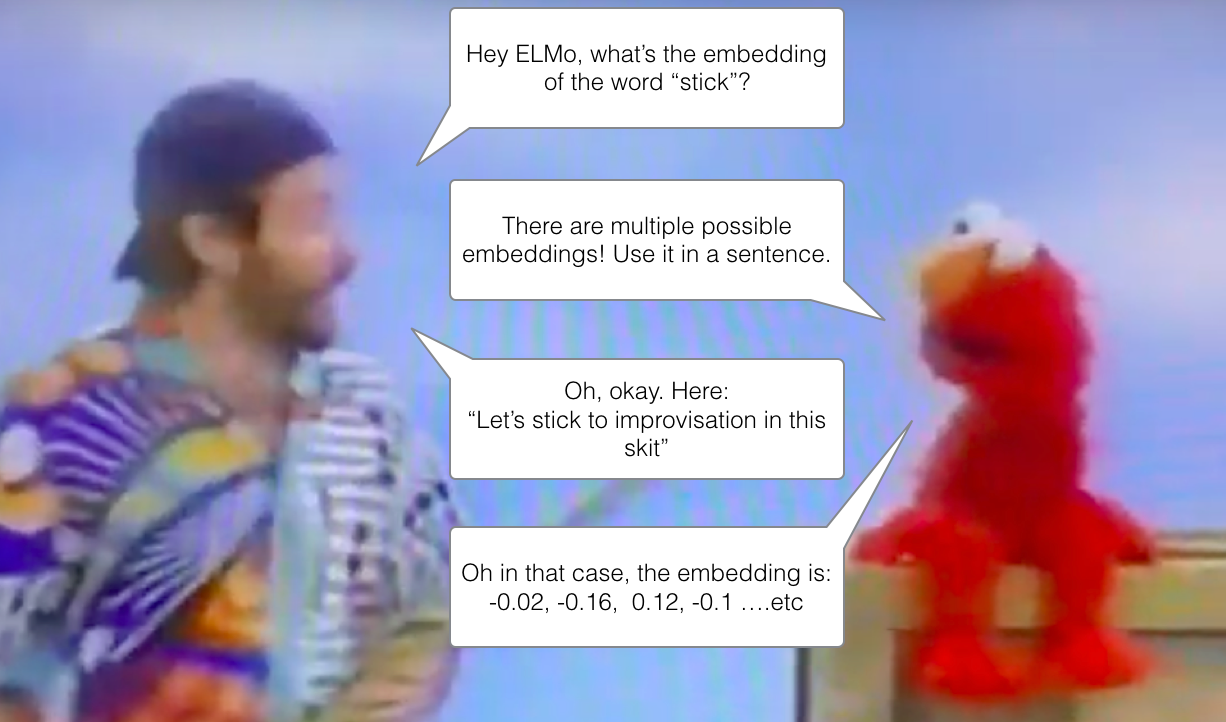
\includegraphics[width=.8\linewidth]{ elmo_and_robby.png}
		\end{center}
\end{frame}


\begin{frame}{ Embeddings from Language Models (ELMo)}
	\begin{center}
		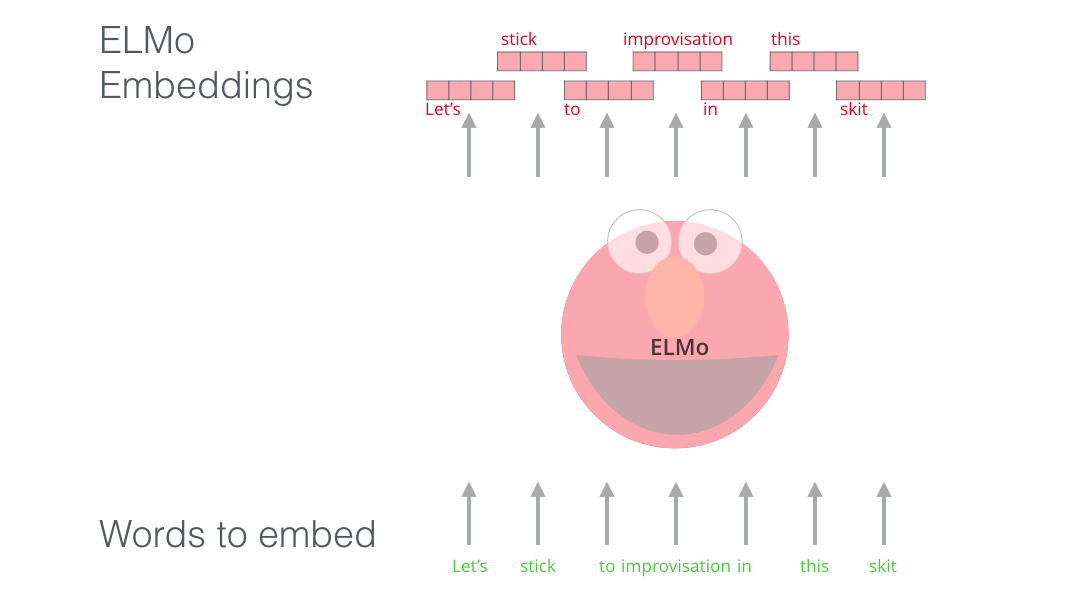
\includegraphics[width=.8\linewidth]{elmo1.png}
	\end{center}
	\vfill
	\footnotesize
	{\color{blue} \url{https://jalammar.github.io/illustrated-bert/}  } 
\end{frame}


\begin{frame}{ Embeddings from Language Models (ELMo)}
	\begin{center}
		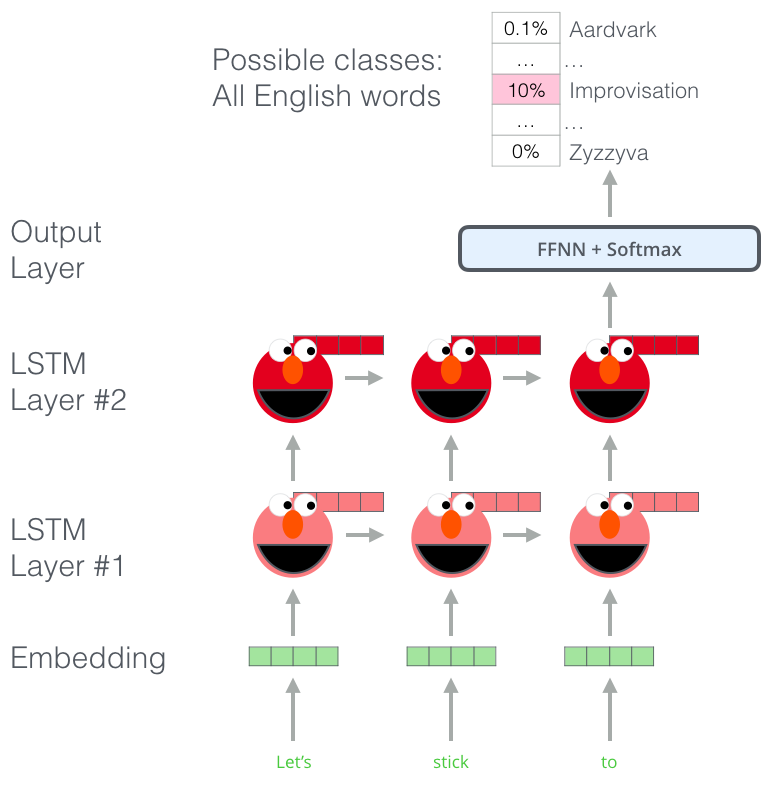
\includegraphics[width=.5\linewidth]{elmo2.png}
	\end{center}
\end{frame}

\begin{frame}{ Embeddings from Language Models (ELMo)}
	\begin{center}
		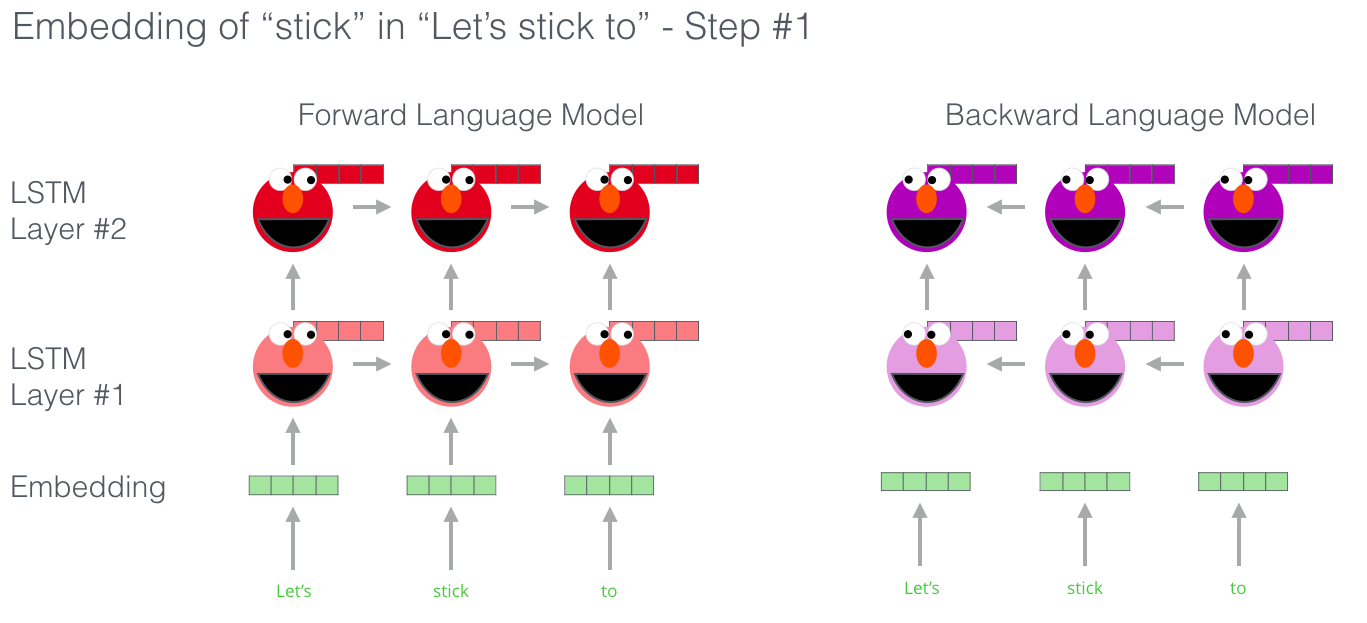
\includegraphics[width=.9\linewidth]{elmo3.png}
	\end{center}
\end{frame}

\begin{frame}{ Embeddings from Language Models (ELMo)}
	\begin{center}
		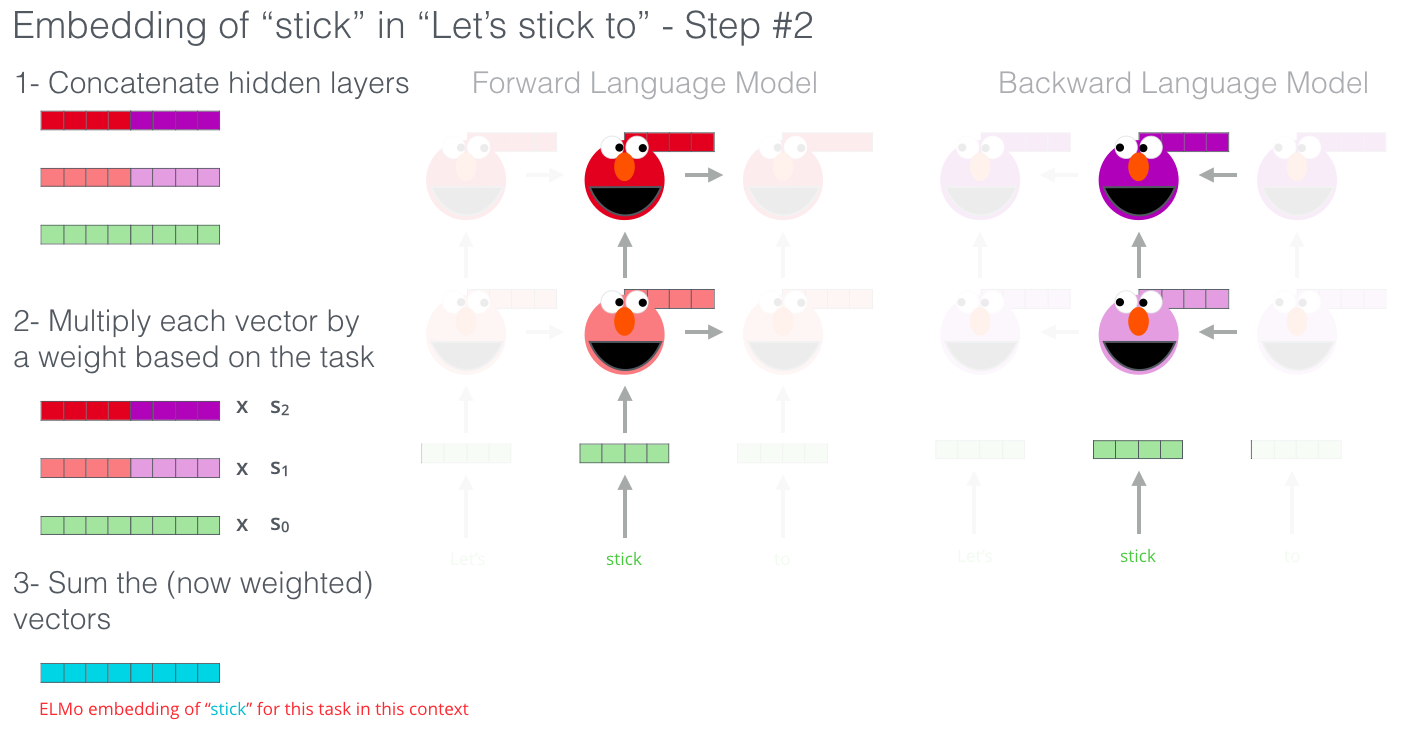
\includegraphics[width=.9\linewidth]{elmo4.png}
	\end{center}
\end{frame}



\begin{frame}{ Embeddings from Language Models (ELMo)}
	\begin{center}
		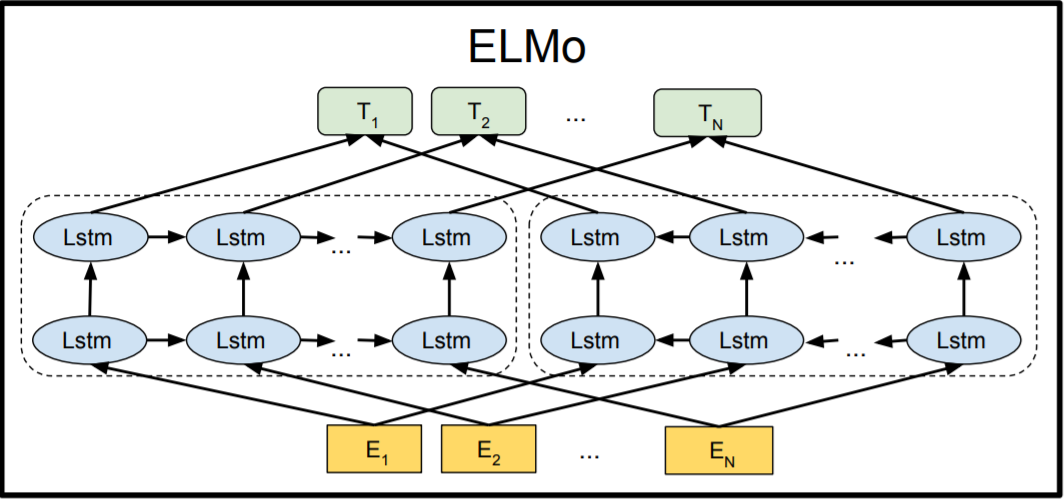
\includegraphics[width=.6\linewidth]{ elmo.png}
	\end{center}
	В качестме эмбеддинга используется вектор $[𝑇 , h_𝑙, h_𝑟]$, где $𝑇$ - токены, которые сетка выплёвывает наружу, $h_𝑙$ - итоговое скрытое состояние ячеек при проходе слева направо, $h_𝑟$ - справа налево.
	\vfill
	\footnotesize
	{\color{blue} \url{https://arxiv.org/pdf/1802.05365.pdf}  } 
\end{frame}


\begin{transitionframe}
	\begin{center}
			\Huge  DSSM
		\end{center}
\end{transitionframe}


\begin{frame}{Рекомендательные системы}
\begin{center}
	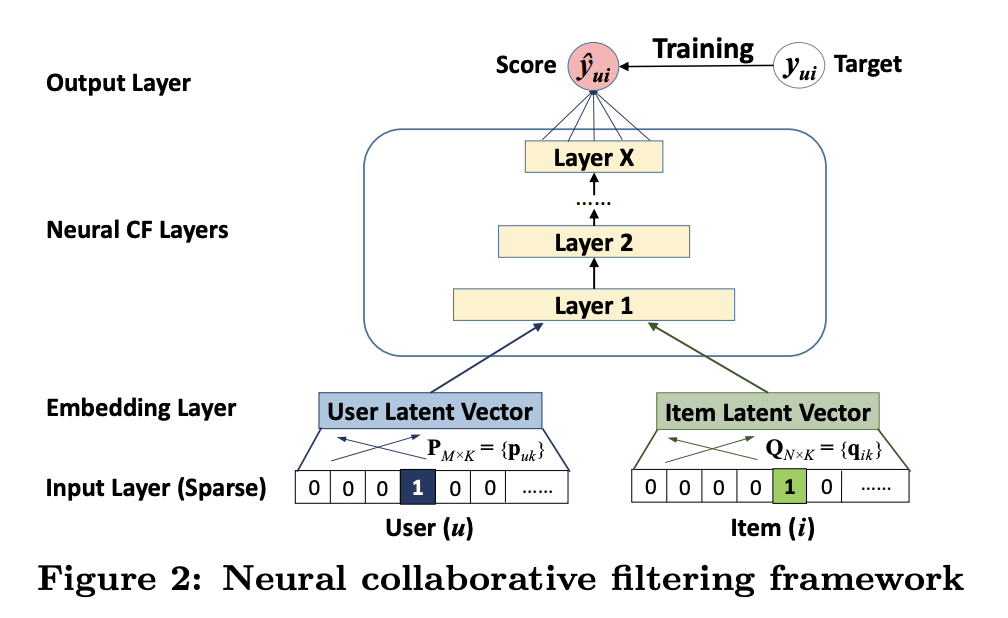
\includegraphics[width=.7\linewidth]{colab_filtering.png}
\end{center}
	\vfill
\footnotesize
{\color{blue} \url{https://arxiv.org/pdf/1708.05031.pdf}  } 
\end{frame}



\end{document}
